\documentclass[twoside,11pt]{article}

% ? Specify used packages
\usepackage{graphicx}        %  Use this one for final production.
% \usepackage[draft]{graphicx} %  Use this one for drafting.
% ? End of specify used packages

% Nice fonts -- during development.
%\usepackage{fancyheadings}
%\usepackage[latin1]{inputenc}
%\usepackage{ae}
%\usepackage{cmbright}

\pagestyle{myheadings}
\raggedbottom

% -----------------------------------------------------------------------------
% ? Document identification
% Fixed part
\newcommand{\stardoccategory}  {Programming User Note}
\newcommand{\stardocinitials}  {PROG}
\newcommand{\stardocsource}    {PRG\stardocnumber}
\newcommand{\stardoccopyright}
{Copyright \copyright\ 2001 Council for the Central Laboratory of the
Research Councils}

% Variable part - replace [xxx] as appropriate.
\newcommand{\stardocnumber}    {1.1}
\newcommand{\stardocauthors}   {Peter W. Draper}
\newcommand{\stardocdate}      {21 December 2001}
\newcommand{\stardoctitle}     {SPLAT - A Spectral Analysis Tool}
\newcommand{\stardocversion}   {1.0}
\newcommand{\stardocmanual}    {Provisional Programmers' Manual}
\newcommand{\stardocabstract}  {
\textsf{SPLAT} is an extensible analysis and display tool for extracted
spectra. This document describes some information that is expected to
be useful when extending \textsf{SPLAT}.
}
% ? End of document identification
% -----------------------------------------------------------------------------

% +
%  Name:
%     sun.tex
%
%  Purpose:
%     Template for Starlink User Note (SUN) documents.
%     Refer to SUN/199
%
%  Authors:
%     AJC: A.J.Chipperfield (Starlink, RAL)
%     BLY: M.J.Bly (Starlink, RAL)
%     PWD: Peter W. Draper (Starlink, Durham University)
%
%  History:
%     17-JAN-1996 (AJC):
%        Original with hypertext macros, based on MDL plain originals.
%     16-JUN-1997 (BLY):
%        Adapted for LaTeX2e.
%        Added picture commands.
%     13-AUG-1998 (PWD):
%        Converted for use with LaTeX2HTML version 98.2 and
%        Star2HTML version 1.3.
%      1-FEB-2000 (AJC):
%        Add Copyright statement in LaTeX
%     {Add further history here}
%
% -

\newcommand{\stardocname}{\stardocinitials /\stardocnumber}
\markboth{\stardocname}{\stardocname}
\setlength{\textwidth}{160mm}
\setlength{\textheight}{230mm}
\setlength{\topmargin}{-2mm}
\setlength{\oddsidemargin}{0mm}
\setlength{\evensidemargin}{0mm}
\setlength{\parindent}{0mm}
\setlength{\parskip}{\medskipamount}
\setlength{\unitlength}{1mm}

% -----------------------------------------------------------------------------
%  Hypertext definitions.
%  ======================
%  These are used by the LaTeX2HTML translator in conjunction with star2html.

%  Comment.sty: version 2.0, 19 June 1992
%  Selectively in/exclude pieces of text.
%
%  Author
%    Victor Eijkhout                                      <eijkhout@cs.utk.edu>
%    Department of Computer Science
%    University Tennessee at Knoxville
%    104 Ayres Hall
%    Knoxville, TN 37996
%    USA

%  Do not remove the %begin{latexonly} and %end{latexonly} lines (used by
%  LaTeX2HTML to signify text it shouldn't process).
%begin{latexonly}
\makeatletter
\def\makeinnocent#1{\catcode`#1=12 }
\def\csarg#1#2{\expandafter#1\csname#2\endcsname}

\def\ThrowAwayComment#1{\begingroup
    \def\CurrentComment{#1}%
    \let\do\makeinnocent \dospecials
    \makeinnocent\^^L% and whatever other special cases
    \endlinechar`\^^M \catcode`\^^M=12 \xComment}
{\catcode`\^^M=12 \endlinechar=-1 %
 \gdef\xComment#1^^M{\def\test{#1}
      \csarg\ifx{PlainEnd\CurrentComment Test}\test
          \let\html@next\endgroup
      \else \csarg\ifx{LaLaEnd\CurrentComment Test}\test
            \edef\html@next{\endgroup\noexpand\end{\CurrentComment}}
      \else \let\html@next\xComment
      \fi \fi \html@next}
}
\makeatother

\def\includecomment
 #1{\expandafter\def\csname#1\endcsname{}%
    \expandafter\def\csname end#1\endcsname{}}
\def\excludecomment
 #1{\expandafter\def\csname#1\endcsname{\ThrowAwayComment{#1}}%
    {\escapechar=-1\relax
     \csarg\xdef{PlainEnd#1Test}{\string\\end#1}%
     \csarg\xdef{LaLaEnd#1Test}{\string\\end\string\{#1\string\}}%
    }}

%  Define environments that ignore their contents.
\excludecomment{comment}
\excludecomment{rawhtml}
\excludecomment{htmlonly}

%  Hypertext commands etc. This is a condensed version of the html.sty
%  file supplied with LaTeX2HTML by: Nikos Drakos <nikos@cbl.leeds.ac.uk> &
%  Jelle van Zeijl <jvzeijl@isou17.estec.esa.nl>. The LaTeX2HTML documentation
%  should be consulted about all commands (and the environments defined above)
%  except \xref and \xlabel which are Starlink specific.

\newcommand{\htmladdnormallinkfoot}[2]{#1\footnote{#2}}
\newcommand{\htmladdnormallink}[2]{#1}
\newcommand{\htmladdimg}[1]{}
\newcommand{\hyperref}[4]{#2\ref{#4}#3}
\newcommand{\htmlref}[2]{#1}
\newcommand{\htmlimage}[1]{}
\newcommand{\htmladdtonavigation}[1]{}

\newenvironment{latexonly}{}{}
\newcommand{\latex}[1]{#1}
\newcommand{\html}[1]{}
\newcommand{\latexhtml}[2]{#1}
\newcommand{\HTMLcode}[2][]{}

%  Starlink cross-references and labels.
\newcommand{\xref}[3]{#1}
\newcommand{\xlabel}[1]{}

%  LaTeX2HTML symbol.
\newcommand{\latextohtml}{\LaTeX2\texttt{HTML}}

%  Define command to re-centre underscore for Latex and leave as normal
%  for HTML (severe problems with \_ in tabbing environments and \_\_
%  generally otherwise).
\renewcommand{\_}{\texttt{\symbol{95}}}

% -----------------------------------------------------------------------------
%  Debugging.
%  =========
%  Remove % on the following to debug links in the HTML version using Latex.

% \newcommand{\hotlink}[2]{\fbox{\begin{tabular}[t]{@{}c@{}}#1\\\hline{\footnotesize #2}\end{tabular}}}
% \renewcommand{\htmladdnormallinkfoot}[2]{\hotlink{#1}{#2}}
% \renewcommand{\htmladdnormallink}[2]{\hotlink{#1}{#2}}
% \renewcommand{\hyperref}[4]{\hotlink{#1}{\S\ref{#4}}}
% \renewcommand{\htmlref}[2]{\hotlink{#1}{\S\ref{#2}}}
% \renewcommand{\xref}[3]{\hotlink{#1}{#2 -- #3}}
%end{latexonly}
% -----------------------------------------------------------------------------
% ? Document specific \newcommand or \newenvironment commands.

% SPLAT.
\newcommand{\SPLAT}{\textsf{SPLAT}}

% Major graphic (like a screen shot). Needs ".gif" and ".eps" forms.
% \latexhtml{\includegraphics[width=4.5in]{#1.eps}}{\htmladdimg{#1.gif}}
\newcommand{\mainfigure}[1]
{\begin{center}
 \latexhtml{\includegraphics[scale=0.5]{#1.eps}}{\htmladdimg{#1.gif}}
 \end{center}
}

\newcommand{\clippedmainfigure}[1]
{\begin{quote}
 \latexhtml{\includegraphics[scale=0.5,clip=true]{#1.eps}}{\htmladdimg{#1.gif}}
 \end{quote}
}

% Inline a graphic (like an icon). Needs ".gif" and ".eps" forms.
\newcommand{\inline}[1]
        {\latexhtml{\includegraphics[scale=0.5]{#1.eps}}
        {\htmladdimg[align=center]{#1.gif}}}

% UI elements.
\newcommand{\menuitem}[1]{\textbf{#1}}
\newcommand{\submenuitem}[2]{\latexhtml{\textbf{#1$\rightarrow$#2}}{\textbf{#1=>#2}}}
\newcommand{\labelitem}[1]{\textbf{#1}}

% typed text.
\newcommand{\hitext}[1]{\texttt{#1}}

% i.e.
\newcommand{\ie}{\textit{i.e.}}

% e.g..
\newcommand{\eg}{\textit{e.g.}}

% etc.
\newcommand{\etc}{\textit{etc.}}

% Heading for a paragraph section.
\newcommand{\subheading}[1]{\textbf{\large{#1}}}

% Heading for example code.
\newcommand{\exampleheading}[1]
{\begin{center}
  \fbox{#1}
 \end{center}
}

% +
%  Name:
%     apidocs_formatted.tex
%     sun.tex
%
%  Purpose:
%     Defines LaTeX (and Star2HTML) commands for laying out Java
%     documentation from my version of the docletLatex doclet.
%
%  Authors:
%     PWD: Peter W. Draper (Starlink, Durham University)
%
%  History:
%     05-DEC-2001 (PWD):
%        Original version.
%     {Add further history here}
%
% -
\newcommand{\entityintro}[3]{
  \htmlref{\textbf{\Large{#1}}}{#2}
  \dotfill\pageref{#2}
  \begin{quote}
  #3
  \end{quote}
}

\newcommand{\refdefined}[1]{}

\newcommand{\startsection}[4]{
   \subsubsection{\label{#3}{#2}}
   #4
}

\newcommand{\startsubsubsection}[1]{
   \begin{quote}
   \textbf{\large{#1}}
   \end{quote}
}

\newcommand{\method}[1]{\texttt{#1}}

\newenvironment{desc}{\begin{quote}}{\end{quote}}

\newcommand{\constructors}{
   \par\textbf{\large{Constructors}}\\
   \hrule
}

\newcommand{\methods}{
   \par\textbf{\large{Methods}}\\
   \hrule
}

\newcommand{\inherited}[1]{
   \par\textbf{\large{Methods inherited from class #1}}\\
   \hrule
}

\newcommand{\fields}[1]{
   \par\textbf{\large{#1}}\\
   \hrule
}

\newcommand{\field}[2]{
   \par\texttt{#1}
   \begin{itemize}
   \item #2
   \end{itemize}
}

% ? End of document specific commands
% -----------------------------------------------------------------------------
%  Title Page.
%  ===========
\renewcommand{\thepage}{\roman{page}}
\begin{document}
\thispagestyle{empty}

%  Latex document header.
%  ======================
\begin{latexonly}
   CCLRC / \textsc{Rutherford Appleton Laboratory} \hfill \textbf{\stardocname}\\
   {\large Particle Physics \& Astronomy Research Council}\\
   {\large Starlink Project\\}
   {\large \stardoccategory\ \stardocnumber}
   \begin{flushright}
   \stardocauthors\\
   \stardocdate
   \end{flushright}
   \vspace{-4mm}
   \rule{\textwidth}{0.5mm}
   \vspace{5mm}
   \begin{center}
      {\LARGE\textbf{\stardoctitle \\ [2.5ex]}}
   \end{center}
   \vspace{5mm}

% ? Add picture here if required for the LaTeX version.
\begin{center}
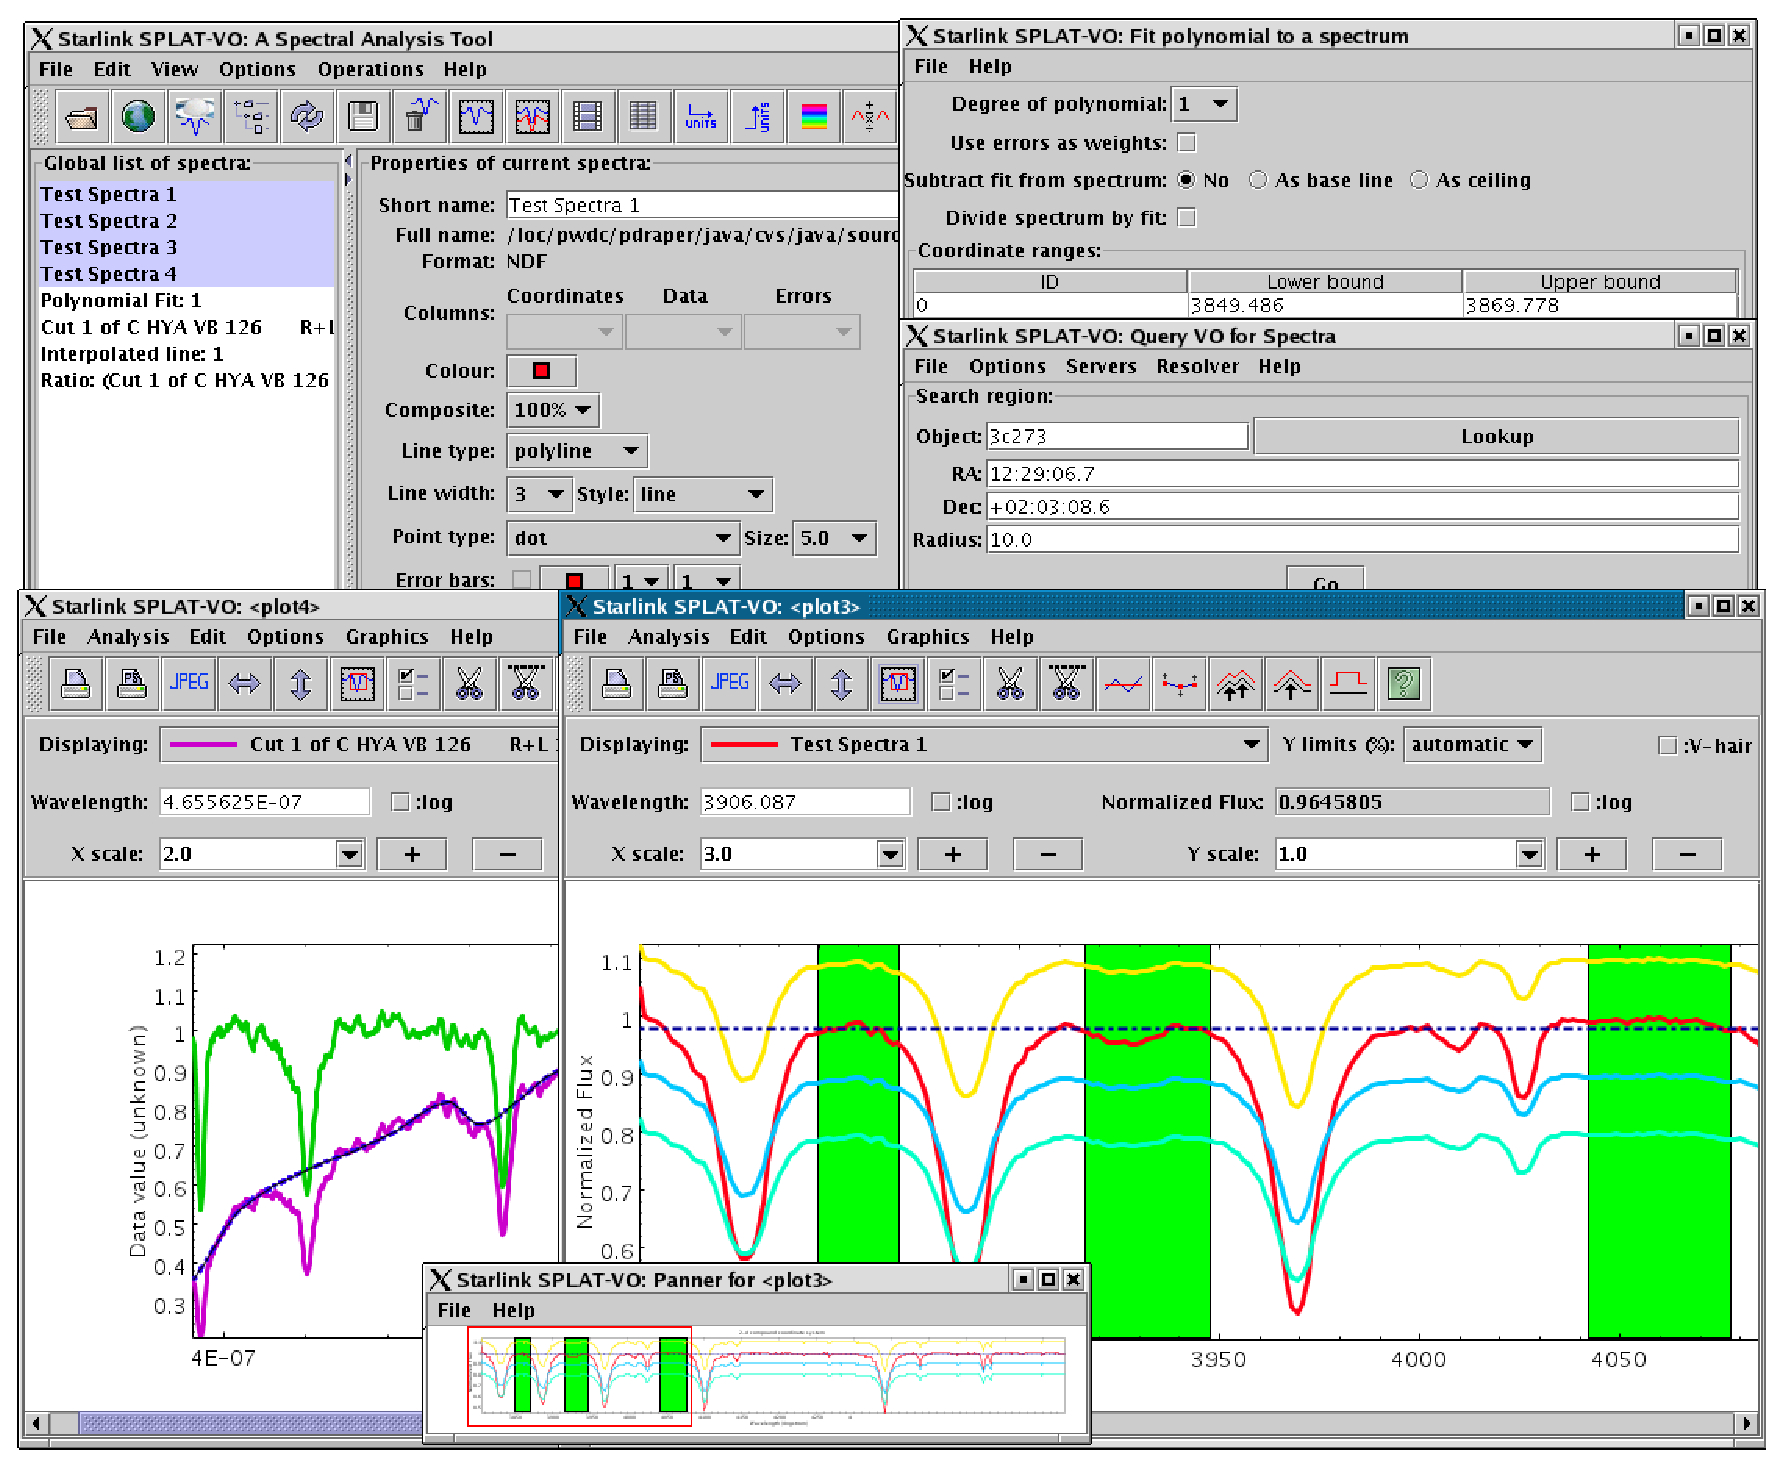
\includegraphics[scale=0.6]{sun243_figures/frontfigure.eps}
\end{center}
% ? End of picture

% ? Heading for abstract if used.
   %\vspace{10mm}
   \begin{center}
      {\Large\textbf{Abstract}}
   \end{center}
% ? End of heading for abstract.
\end{latexonly}

%  HTML documentation header.
%  ==========================
\begin{htmlonly}
   \xlabel{}
   \begin{rawhtml} <H1 ALIGN=CENTER> <FONT COLOR="#000099">\end{rawhtml}
      \stardoctitle
   \begin{rawhtml} </FONT></H1> \end{rawhtml}

% ? Add picture here if required for the hypertext version.
   \begin{center}
      \htmladdimg{frontfigure.jpg}
   \end{center}
% ? End of picture

   \begin{rawhtml} <P> <I> \end{rawhtml}
   \stardoccategory\ \stardocnumber \\
   \stardocauthors \\
   \stardocdate
   \begin{rawhtml} </I> </P> <H3> \end{rawhtml}
      \htmladdnormallink{CCLRC / Rutherford Appleton Laboratory}
                        {http://www.cclrc.ac.uk} \\
      \htmladdnormallink{Particle Physics \& Astronomy Research Council}
                        {http://www.pparc.ac.uk} \\
   \begin{rawhtml} </H3> <H2> \end{rawhtml}
      \htmladdnormallink{Starlink Project}{http://www.starlink.rl.ac.uk/}
   \begin{rawhtml} </H2> \end{rawhtml}
   \htmladdnormallink{\htmladdimg{source.gif} Retrieve hardcopy}
      {http://www.starlink.rl.ac.uk/cgi-bin/hcserver?\stardocsource}\\

%  HTML document table of contents.
%  ================================
%  Add table of contents header and a navigation button to return to this
%  point in the document (this should always go before the abstract \section).
  \label{stardoccontents}
  \begin{rawhtml}
    <HR>
    <H2>Contents</H2>
  \end{rawhtml}
  \htmladdtonavigation{\htmlref{\htmladdimg{contents_motif.gif}}
        {stardoccontents}}

% ? New section for abstract if used.
  \section{\xlabel{abstract}Abstract}
% ? End of new section for abstract
\end{htmlonly}

% -----------------------------------------------------------------------------
% ? Document Abstract. (if used)
%  ==================
\begin{center}
\stardocabstract
\end{center}
% ? End of document abstract

% -----------------------------------------------------------------------------
% ? Latex Copyright Statement
%  =========================
\begin{latexonly}
\newpage
\vspace*{\fill}
\stardoccopyright
\end{latexonly}
% ? End of Latex copyright statement

% -----------------------------------------------------------------------------
% ? Latex document Table of Contents (if used).
%  ===========================================
\newpage
\begin{latexonly}
  \setlength{\parskip}{0mm}
  \tableofcontents
  \setlength{\parskip}{\medskipamount}
  \markboth{\stardocname}{\stardocname}
\end{latexonly}
% ? End of Latex document table of contents
% -----------------------------------------------------------------------------

\cleardoublepage
\renewcommand{\thepage}{\arabic{page}}
\setcounter{page}{1}

% ? Main text

\section{Introduction\xlabel{introduction}}

This manual is an provisional extension to
\xref{SUN/243}{sun243}{}. It describes some of the information
required to extend \SPLAT\ using plugins, remote-control and from
command-line scripts.

\section{Extending \SPLAT}

\SPLAT\ is written in Java (with some JNI interface code to access the
Starink NDF and AST libraries) and has a scripting component called
\htmladdnormallinkfoot{BeanShell}{http://www.beanshell.org}
embedded in it. This provides two useful resources, the ability to
extend \SPLAT\ dynamically and to make it respond to remote
control commands.

Extending \SPLAT\ dynamically is done by two orthogonal methods, by
`plugins' that are loaded during startup (and are then just part of
\SPLAT) and by using \SPLAT\ as a
library of routines that you use from your own BeanShell scripts.

Note that if you are thinking about extending \SPLAT\ then you will
need to be familiar with Java and BeanShell (BeanShell uses a Java
syntax and has the full Java APIs available to it, so the first
condition mostly implies the latter, one of the reasons for choosing
BeanShell). Also \SPLAT\ is very likely to change considerably (\ie\
the internal APIs cannot be relied on) so don't do anything too
serious without contacting the support programmer.

\subsection{Plugins}

A plugin can be either a very simple piece of code or a full toolbox
that integrates into \SPLAT\ much like the existing ones do.

As a simple example let's say that you'd always like to load a certain
list of spectra into \SPLAT\ each time it starts up. To do this you
need to create a BeanShell script, say called
\hitext{splat\_loads.bsh}, and add the following text to it:
\begin{quote}
\begin{verbatim}
print( "Loading the default list of spectra" );
browser.displaySpectrum( "spectrum1.sdf" );
browser.displaySpectrum( "spectrum2.sdf" );
browser.displaySpectrum( "spectrum3.sdf" );
\end{verbatim}
\end{quote}
Naturally you need to modify the names of the spectra to some of your
own. Now to get this plugin to be actually run by \SPLAT\ do the
following (assumes you're using the C-shell):
\begin{quote}
\begin{verbatim}
% setenv SPLAT_PLUGINS splat_loads.bsh
\end{verbatim}
\end{quote}
and then just start up \SPLAT. You should then see it start up saying
something like:
\begin{quote}
\begin{verbatim}
Remote control established
BeanShell plugins...
Loading: splat_loads.bsh
Loading the default list of spectra
\end{verbatim}
\end{quote}
and your spectra should be added to the global list and displayed in a
plot.

One thing to take a good look at in the BeanShell code above is the
reference to \hitext{browser}. This is a variable that's available to
all plugins and is actually a reference to the browser window object
(which is an instance of a class called \hitext{SplatBrowser}). So
using this reference you can do almost anything that the browser
window can do. More specifically you can use any of the public methods
of the \hitext{SplatBrowser} class. More of the public methods of
\hitext{SplatBrowser} are shown later.

The following code (from the example
\hitext{\$SPLAT\_DIR/example\_plugin3.bsh}) extends the idea of
automatically displaying spectra when \SPLAT\ starts up to something
more flexible. It looks for a file \hitext{.splat\_autoloads} in the
current directory and if found reads the lines (each of which are
assumed to contain a file name) from it to construct a list of spectra
to display. If the file only has one line ``*'' then all the NDFs are
automatically loaded.

\exampleheading{Example spectral auto-loading}

\begin{verbatim}
/**
 * Name:
 *    example_plugin3.bsh
 *
 * Purpose:
 *    Demonstrate auto-load of local files into SPLAT on startup.
 *
 * Usage:
 *    setenv SPLAT_PLUGINS \$SPLAT_DIR/example_plugin3.bsh
 *
 * Description:
 *    This BeanShell script is an example plugin for SPLAT. It
 *    looks for the file ".splat_autoloads" in the current directory
 *    and arranges for any files listed in it to be automatically loaded
 *    into SPLAT. If the file contains the single entry "*", then all
 *    spectra in the directory are loaded.
 *
 * Language:
 *    BeanShell
 */

// Startup message.
print( "Checking for autoloads" );

// Name of the autoload file.
AUTO_LOAD_FILE = ".splat_autoloads";

// Types of spectra to autoload (used for the special wildcard pattern).
FILE_PATTERN = "sdf";

// Check for the autoload file.
filePath = pathToFile( AUTO_LOAD_FILE );
if ( ! filePath.exists() || ! filePath.canRead() || ! filePath.isFile() ) {
    print( "No autoloads found" );
    return;
}

// Open the auto load file for reading (wraps an input file stream in
// a buffered reader, so we can read it line-by-line).
inStream = new FileInputStream( filePath );
inReader = new InputStreamReader( inStream );
bufReader = new BufferedReader( inReader );

// Read the auto load file contents in a space separated String.
concat = new StringBuffer();
fileCount = 0;
while ( ( line = bufReader.readLine() ) != null ) {
   concat.append( line ).append( " " );
   fileCount++;
}
names = concat.substring( 0, concat.length() - 1 );

// Close the input streams and readers.
inStream.close();
inReader.close();
bufReader.close();

// If no lines were found, then do nothing.
if ( fileCount == 0 ) {
    print( "Autoload file is empty" );
    return;
}

// If fileCount is 1 it could be the special pattern "*".
if ( fileCount == 1 && "*".equals( names ) ) {
    print( "Will auto load all local spectra" );

    // Need to get a list of all spectra in this directory. To make
    // this quick use the SPLAT class SpectralFileFilter (assumes
    // SPLAT classes are on CLASSPATH, they will be for a plugin).
    import uk.ac.starlink.splat.util.SpectralFileFilter;
    fileFilter = new SpectralFileFilter( FILE_PATTERN );
    list = filePath.getParentFile().listFiles( fileFilter );

    // If no files were found, give up.
    fileCount = list.length;
    if ( fileCount == 0 ) {
        print( "No spectra are available in the directory" );
        return;
    }

    // Now create the list of space seperated names.
    concat = new StringBuffer();
    for ( int i = 0; i < fileCount; i++ ) {
        concat.append( list[i].getPath() ).append( " " );
    }
    names = concat.substring( 0, concat.length() - 1 );
}

// If we're really in SPLAT display the spectra.
if ( browser != void ) {
    print( "Autoloading local spectra" );
    browser.displaySpectra( names );
} else {
    print( "No browser available" );
}
return;
\end{verbatim}

In this example note how BeanShell works much like Java, except for
its use of dynamically typed objects and the way that you do not need
a class structure. Note also how it is making free use of Java
classes, such as \hitext{String}, \hitext{StringBuffer},
\hitext{FileInputStream}, \hitext{InputStreamReader} and
\hitext{BufferedReader}. There's also a smattering of BeanShell
commands, such as \hitext{print} and \hitext{pathToFile}, both of
which could have been achieved using standard Java commands \\
(\hitext{System.out.println} and \hitext{java.io.File})
instead. The list of built-in BeanShell commands is described
\latexhtml{in appendix \ref{beanshell_appendix}}
{\htmlref{later}{beanshell_appendix}}.

The autoloading example is about as complex as a BeanShell script
should get, any more complex and you should really be thinking of
using Java classes. The next example shows how you could do this.
\begin{quote}
\begin{verbatim}
//  Add a directory to the CLASSPATH and load a local class.
addClassPath( ``/my/splat/plugins" );
localClass = new MyLocalClass( browser );
\end{verbatim}
\end{quote}
Which just extends the \hitext{CLASSPATH} used by \SPLAT\ to include
your local root directory and then creates an instance the class that
will do the work. Note that the \hitext{browser} variable is passed
along for accessing the internals of \SPLAT.

A more complete example of this can be found in
\hitext{\$SPLAT\_DIR} in the files \hitext{maths\_plugin.bsh} and
\hitext{BasicMaths.java}. This is actually a simplified version of the
tool that performs maths between pairs of spectra (for the record the
plugin was written first) and reveals some details of how things
really work in \SPLAT.

\subsection{Remote control and command-line display tools}

Using remote control you can pass commands to \SPLAT\ to make it do
simple things like display a spectrum and add a spectrum to a plot. In
fact this is such a useful idea that there are two commands already
available. These are:
\begin{itemize}
\item \hitext{splatdisp}
\item \hitext{splatdispmany}
\end{itemize}
The first command takes the name of a spectrum and adds it to a plot,
if a plot identifier is given (this is the \hitext{n} in any names
like \hitext{<plotn>} that you see), or just displays it in a new
plot. The second command takes a list of spectra and displays them all
in a new plot. Either of these scripts should serve as suitable
starting points for any scripts that you'd like to develop (assuming
you want to write these in BeanShell).

Remote control is accessed using a \hitext{ServerSocket} that listens
on a randomly chosen port of the machine that \SPLAT\ is running
on. Behind the \hitext{ServerSocket} the BeanShell is used to
interpret any commands, so much of what you can do via remote control
is the same as described in the plugins section.

The port number used by \SPLAT\ is written into the file
\hitext{\$HOME/.splat/.remote}, which can only be read by the
owner. The file contains three fields:
\begin{enumerate}
\item the machine internet address
\item the port number
\item a security cookie
\end{enumerate}
When you connect through a port the first message you send should be
the security cookie. If this isn't given or an invalid value is given
then the port is immediately closed. After this is acknowledged you
may go on to give BeanShell commands, as strings, for \SPLAT\ to
interpret.

A couple of useful examples are shown now. The first makes an existing
plot zoom itself to a given X factor and then center itself on a
given wavelength. The second changes the drawing colour of a spectrum.

\exampleheading{Example zoom and centre}
\begin{verbatim}

//${SPLAT_DIR}/splatsh $0 ${1+"$@"}; exit;
// Note first line is blank, do not remove it as this starts "sh", which
// runs the next line, which runs splatsh on this file. This header
// section is ignored as it is a beanshell comment, that "sh" never sees.

/**
 * Name:
 *    zoomandcentre
 *
 * Purpose:
 *    Zoom a SPLAT plot and maybe centre it on a wavelength
 *
 * Usage:
 *    zoomandcentre plot_number x_scale [wavelength]
 *
 * Description:
 *    This command zooms a plot to the given X scale factor and
 *    then, optionally, centres it on a given wavelength.
 *
 * Notes:
 *    This actually reduces to wrapping the following lines
 *    of BeanShell that are evaluated in the remote interpreter:
 *
 *       plotIndex = globallist.getPlotIndex( plotNumber );
 *       plot = globallist.getPlot( plotIndex );
 *       plot.setXScale( scale );
 *       plot.setScale();
 *       plot.centreOnXCoordinate( wavelength );
 *
 *    Where plotNumber, scale and wavelength are the command-line
 *    arguments to this script.
 *
 * Language:
 *    BeanShell (Java-based scripting language).
 */

/**
 * Print the usage message and exit.
 */
usage ()
{
    print( "Usage: zoomandcentre plot_number x_scale [wavelength]" );
    exit();
}

//  Import any classes that we need from SPLAT.
import uk.ac.starlink.splat.util.RemoteUtilities;

/**
 * Open up the connection to SPLAT, this does not return if fails.
 */
openConnection()
{
    //  Read the contact details for the current SPLAT instance. These are
    //  the machine name, the server port and the authentication cookie.
    Object[] contactDetails = RemoteUtilities.readContactFile();

    //  See if SPLAT is around and listening.
    if ( contactDetails == null ||
         ! RemoteUtilities.isListening( contactDetails ) ) {
        print( "Failed to connect to SPLAT" );
        exit();
    }
    return contactDetails;
}

/**
 * Convert the plot identifier into a global index. Also
 * assigns the PlotControl object to the plot variable in the remote
 * interpreter.
 */
getPlot( plotNumber )
{
    // Ask global list for the proper index of the plot. Assigns the
    // result to the variable "plotIndex" in the remote interpreter.
    result = sendCommand
        ( "plotIndex = globallist.getPlotIndex(" + plotNumber + ");"  );

    //  If we get back a "-1" then the plot doesn't exist.
    if ( "-1".equals( result ) ) {
        print( "Failed to find plot (" + plotNumber + ")" );
        exit();
    }
    else {
        // Plot exists, so get the actual object and assign this to
        // the plot variable.
        result = sendCommand( "plot = globallist.getPlot( plotIndex );" );
    }
}

/**
 * Send the command to scale in X.
 */
setScale( scale )
{
    result = sendCommand( "plot.setXScale(" + scale + ");" );
    result = sendCommand( "plot.setScale();" );
}

/**
 * Send the command to centre on a given wavelength.
 */
setCentre( wavelength )
{
    result = sendCommand
        ( "plot.centreOnXCoordinate( \"" + wavelength + "\");" );
}

/**
 * Send a command to SPLAT.
 */
sendCommand( command )
{
    try {
        print( command );
        result = RemoteUtilities.sendRemoteCommand( contactDetails, command );
    }
    catch ( Exception e ) {
        print( "Failed to send command to SPLAT");
        print( e.getMessage() );
    }
    print( "Result = " + result );
    return result;
}

//  Check number of command-line arguments match our expectation.
if ( bsh.args.length > 3 || bsh.args.length < 2 ) {
   usage();
}

//  Contact SPLAT. If successful the contact details are returned.
Object[] contactDetails = openConnection();

//  Make the translation from plot identifier to plot object.
getPlot( bsh.args[0] );

//  Send the scale command.
setScale( bsh.args[1] );

//  Send the centre command.
if ( bsh.args.length == 3  ) {
  setCentre( bsh.args[2] );
}
exit();
\end{verbatim}


This example (and the following one) is written in BeanShell. Note how
the script is wrapped as a bourne shell script by the command on the
second line. The \hitext{splatsh} shell arranges to run this script
using the BeanShell interpreter and also makes sure that 
\SPLAT\ classes are available on the CLASSPATH.

The procedural details of the script are quite simple, it consists of
connect to \SPLAT, get a handle to the plot, and then issue
the commands that perform the scale and optional centering of the
plot.

The most important point to notice is that fully qualified BeanShell
commands are sent to \SPLAT\ and these are interpreted remotely, not
in the local script. Also note that the return from a remote command
is a stringifed (\ie\ \hitext{toString()}) version of the result. This
isn't generally very useful, except for getting status information and
the actual object references \etc\ that are created should be retained
in the remote interpreter (the remote interpreter is persistent and
can be relied on for at least the duration of the connection).

Note also that the \hitext{globallist} variable is a special reference set
within the remote interpreter. This provides access to the object that
contains a list of all the spectra and plots currently activated in
\SPLAT. The type of this object is \hitext{GlobalSpecPlotList}. The
full public API to \hitext{GlobalSpecPlotList} is shown later in this
document.

The example is available as the command \hitext{zoomandcentre} in
\hitext{\$SPLAT\_DIR}.

\exampleheading{Example set colour}
\begin{verbatim}

//${SPLAT_DIR}/splatsh $0 ${1+"$@"}; exit;
// Note first line is blank, do not remove it as this starts "sh", which
// runs the next line, which runs splatsh on this file. This header
// section is ignored as it is a beanshell comment, that "sh" never sees.

/**
 * Name:
 *    setcolour
 *
 * Purpose:
 *    Set the colour of a spectrum loaded into SPLAT.
 *
 * Usage:
 *    setcolour short_name colour
 *
 * Description:
 *    This command contacts SPLAT and asks it to set the colour
 *    of a spectrum that it is displaying.
 *
 *    The possible colours are black, blue, cyan, darkGray,
 *    gray, green, lightGray, magenta, orange, pink, red, white and
 *    yellow. Alternatively you can also give an hexidecimal #RRGGBB
 *    integer.
 *
 * Language:
 *    BeanShell (Java-based scripting language).
 */

/**
 * Print the usage message and exit.
 */
usage ()
{
    print( "Usage: setcolour short_name colour" );
    exit();
}

//  Import any classes that we need from SPLAT.
import uk.ac.starlink.splat.util.RemoteUtilities;

/**
 * Open up the connection to SPLAT, this does not return if fails.
 */
openConnection()
{
    //  Read the contact details for the current SPLAT instance. These are
    //  the machine name, the server port and the authentication cookie.
    Object[] contactDetails = RemoteUtilities.readContactFile();

    //  See if SPLAT is around and listening.
    if ( contactDetails == null ||
         ! RemoteUtilities.isListening( contactDetails ) ) {
        print( "Failed to connect to SPLAT" );
        exit();
    }
    return contactDetails;
}

/**
 * Send a command to SPLAT.
 */
sendCommand( command )
{
    try {
        result = RemoteUtilities.sendRemoteCommand( contactDetails, command );
    }
    catch ( Exception e ) {
        print( "Failed to send command to SPLAT");
        print( e.getMessage() );
    }
    return result;
}

/**
 * Convert the spectrum short name into a reference to the SpecData
 * object. This is assigned to the variable "spectrum" in the remote
 * interpreter.
 */
getSpectrum( shortName )
{
    result = sendCommand
        ( "specIndex = globallist.getSpectrumIndex(\"" + shortName + "\");" );

    //  If we get back a "-1" then the spectrum doesn't exist.
    if ( "-1".equals( result ) ) {
        print( "Failed to find spectrum: " + shortName );
        exit();
    }
    result = sendCommand
        ( "spectrum = globallist.getSpectrum( specIndex );" );
}

/**
 * Set the spectrum colour. Must be a java.awt.Color.<name> static method
 * or an RGB integer.
 */
setColour( colour )
{
    try {
        newColour = eval( "Color." + colour );
    }
    catch (Exception e) {
        //  Failed try an integer.
        try {
            newColour = Color.decode( colour );
        }
        catch (Exception ee) {
            print( "Failed to interpret '" + colour + "' as a colour");
            exit();
        }
    }

    //  Convert colour into an RGB integer and issue command to change
    //  it.
    iColour = newColour.getRGB();
    sendCommand( "globallist.setKnownNumberProperty( spectrum, " +
                 "spectrum.LINE_COLOUR, new Integer(" + iColour + ") )" );

}

//  Check number of command-line arguments match our expectation.
if ( bsh.args.length != 2 ) {
   usage();
}

//  Contact SPLAT. If successful the contact details are returned.
Object[] contactDetails = openConnection();

//  Make sure our spectrum exists and make a reference to it.
getSpectrum( bsh.args[0] );

//  Apply the colour.
setColour( bsh.args[1] );

exit();
\end{verbatim}

Again this example is found in \hitext{\$SPLAT\_DIR}, together with a
more extended one called \hitext{setproperty}, which also allows you
to set the line thickness, type and style, as well as whether to
display error bars.

\hitext{\$SPLAT\_DIR} also contains several command-line scripts that
only make use of \SPLAT\ classes. These are, \hitext{fitgauss},
\hitext{fitgauss2} and \hitext{linepositions}, which as you might
expect fit gaussians to lines and just locate accurate line positions
from a initial list. If you need a generally useful similar script
that brings \SPLAT\ functionality to the command-line, then contact
the support programmer. Writing one yourself is probably not possible
at present (mainly because of the need to know more than is outlined
in this document about the internal API structure).

\newpage
\appendix

\section{API documentation\label{api_docs}}

This appendix details the public interfaces of several useful classes
used in \SPLAT (they are a very small sample). They cover all the
requirements of the plugin and remote control scripts outlined
earlier. So you can open, manipulate, create and display spectra
stored in the supported data formats, and trivally contact \SPLAT\
though its socket interface.

Documentation about the full API may be made available at a later
date, but I doubt it.

\subsection{Package uk.ac.starlink.splat.data}

%\vspace{.13in}
%\hbox{\textbf{Classes}}
%\vspace{.13in}
\entityintro{MEMSpecDataImpl}{l0}{This class provides an
implementation of SpecDataImpl to access spectra stored in existing memory.}
\entityintro{SpecData}{l1}{SpecData defines an interface for general
access to spectral datasets of differing fundamental data types and is
the main data model used in SPLAT.}
\entityintro{SpecDataFactory}{l2}{This class creates and clones
instances of SpecData that are appropriate to the data format of the
given spectrum specification.} 
\clearpage
%\subsubsection{Classes}
\startsection{Class}{MEMSpecDataImpl}{l0}
\fbox{\parbox{\textwidth}{
\textit{public class MEMSpecDataImpl extends SpecDataImpl}
}} % end fbox

%\vspace{.09in}

{This class provides an implementation of SpecDataImpl to access
 spectra stored in existing memory. All values are copied into
 arrays stored in memory.

 The main use of this class is for temporary, generated and copied
 spectra.}
\constructors
\method{public \textbf{MEMSpecDataImpl}(\texttt{String} \textbf{name})\label{l3}\label{l4}}
\begin{desc}Constructor - just take a symbolic name for the spectrum, no
 other significance.
\begin{itemize}
\item{Parameter
  \begin{description}
   \item[\textbf{name}]{a symbolic name for the spectrum.}
  \end{description}}
\end{itemize}
\end{desc}

\method{public \textbf{MEMSpecDataImpl}(\texttt{String} \textbf{name}, \texttt{SpecData} \textbf{spectrum})\label{l5}\label{l6}}
\begin{desc}Constructor, clone from another spectrum.
\begin{itemize}
\item{Parameters
  \begin{description}
   \item[\textbf{name}]{a symbolic name for the spectrum.}
   \item[\textbf{spectrum}]{a SpecData object to copy.}
  \end{description}}
\end{itemize}
\end{desc}

\methods
\method{public long \textbf{getAst}()\label{l7}\label{l8}}
\begin{desc}Return reference to AST frameset that defines the coordinate
 relations used by this spectrum.
\begin{itemize}
\item{Returns reference to a raw AST frameset. }
\end{itemize}
\end{desc}

\method{public double \textbf{getData}()\label{l9}\label{l10}}
\begin{desc}Return a copy of the spectrum data values.
\begin{itemize}
\item{Returns reference to the spectrum data values. }
\end{itemize}
\end{desc}

\method{public double \textbf{getDataErrors}()\label{l11}\label{l12}}
\begin{desc}Return a copy of the spectrum data errors.
\begin{itemize}
\item{Returns reference to the spectrum data values. }
\end{itemize}
\end{desc}

\method{public String \textbf{getDataFormat}()\label{l13}\label{l14}}
\begin{desc}Return the data format.
\begin{itemize}
\item{Returns the String "MEMORY". }
\end{itemize}
\end{desc}

\method{public int \textbf{getDims}()\label{l15}\label{l16}}
\begin{desc}Return the data array dimensionality (always length of
 spectrum).
\begin{itemize}
\item{Returns integer array of size 1 returning the number of data
                 values available. }
\end{itemize}
\end{desc}

\method{public String \textbf{getFullName}()\label{l17}\label{l18}}
\begin{desc}Return the full name of spectrum. For memory spectra this has
 no real meaning (i.e. no disk file or URL) so always returns a
 string reminding users that they need to save it.
\begin{itemize}
\item{Returns the String "Memory spectrum". }
\end{itemize}
\end{desc}

\method{public String \textbf{getShortName}()\label{l19}\label{l20}}
\begin{desc}Return a symbolic name.
\begin{itemize}
\item{Returns a symbolic name for the spectrum. Based on the filename. }
\end{itemize}
\end{desc}

\method{public void \textbf{save}()\label{l21}\label{l22}}
\begin{desc}Save is just a copy for this class.
\begin{itemize}
\item{{Exceptions}
  \begin{itemize}
   \item{\vspace{-.6ex}\texttt{SplatException} - never thrown for this implementation.}
  \end{itemize}
}
\end{itemize}
\end{desc}

\method{public void \textbf{setData}(\texttt{double[]} \textbf{data}, \texttt{double[]} \textbf{coords})\label{l23}\label{l24}}
\begin{desc}Set the spectrum data. No errors.
\begin{itemize}
\item{Parameters
  \begin{description}
   \item[\textbf{data}]{the spectrum data values.}
   \item[\textbf{coords}]{the spectrum coordinates, one per data value.}
  \end{description}}
\end{itemize}
\end{desc}

\method{public void \textbf{setData}(\texttt{double[]} \textbf{data}, \texttt{double[]} \textbf{coords}, \texttt{double[]} \textbf{errors})\label{l25}\label{l26}}
\begin{desc}Set the spectrum data. With errors.
\begin{itemize}
\item{Parameters
  \begin{description}
   \item[\textbf{data}]{the spectrum data values.}
   \item[\textbf{coords}]{the spectrum coordinates, one per data value.}
   \item[\textbf{errors}]{the errors of the spectrum data values.}
  \end{description}}
\end{itemize}
\end{desc}

\startsection{Class}{SpecData}{l1}

\fbox{\parbox{\textwidth}{
\textit{public
 class SpecData implements SpecDataAccess, AnalyticSpectrum, java.io.Serializable}
}} % end fbox



%\vspace{.09in}


{SpecData defines an interface for general access to spectral
 datasets of differing fundamental data types and is the main data
 model used in SPLAT.

 It uses a derived class of SpecDataImpl to a supported data format
 (i.e. FITS, NDF and text files) to give generalised access to:
 \begin{itemize}

   \item{ the spectrum data
   }
\item{ the associated data errors
   }
\item{ the coordinate of any data point
   }
\item{ the spectrum properties (i.e. related values)
 }
\end{itemize}


 It should always be used when dealing with spectral data to avoid
 any specialised knowledge of the data format.

 Missing data, or gaps in the spectrum, are indicated using the
 special value SpecData.BAD. Generally useful code should always
 test for this in the data values (otherwise you'll see numeric
 problems as BAD is the lowest possible double value).

 Matching of data values between this spectrum and anothers
 coordinates can currently be done using the evalYData and
 evalYDataArray method of the AnalyticSpectrum interface (but note
 that at present this uses a simple interpolation scheme, so
 shouldn't be used for analysis, except when the interpolated
 spectrum is an analytic one, such as a polynomial).

 Each object records a series of properties that define how the
 spectrum should be rendered (i.e. line colour, thickness, style,
 plotting style, whether to show an errors as bars etc.). These are
 stored in any serialized versions of this class. Rendering using
 the Grf object primitives is performed by this class for spectra
 and error bars.

 Facilities to store the association between this spectrum and the
 various plots that it is currently associated with are also provided
 (but see the SpecList or GlobalSpecPlotList classes for ways to
 structure the control of many spectra, or many spectra and many
 plots).

 General utilities for converting coordinates and looking up values
 are provided, as are methods for specialised functions like
 formatting and unformatting values. This allows you to avoid
 understanding what is returned as a value from a user
 interaction as formatting and unformatting match the units of the
 spectral axes (which can therefore be in esoteric units, like RA
 or Dec).}
\fields{Fields}
\field{public static final double \textbf{BAD}}{Value of BAD (missing) data.}
\field{public static final int \textbf{LINE\_THICKNESS}}{Set or query line thickness.}
\field{public static final int \textbf{LINE\_STYLE}}{Set or query line drawing style.}
\field{public static final int \textbf{LINE\_COLOUR}}{Set or query line colour.}
\field{public static final int \textbf{PLOT\_STYLE}}{Set or query line drawing style.}
\field{public static final int \textbf{LINE\_ALPHA\_BLEND}}{Set or query alpha blending fraction.}
\field{public static final int \textbf{ERROR\_COLOUR}}{Set or query error bar colour.}
\field{public static final int \textbf{POLYLINE}}{Use polyline plotting style.}
\field{public static final int \textbf{HISTOGRAM}}{Use histogram plotting style.}
\field{public static final int \textbf{UNCLASSIFIED}}{Spectrum is unclassified.}
\field{public static final int \textbf{TARGET}}{Spectrum is a target (observation).}
\field{public static final int \textbf{ARC}}{Spectrum is an arc.}
\field{public static final int \textbf{SKY}}{Spectrum is a twilight sky exposure.}
\field{public static final int \textbf{POLYNOMIAL}}{Spectrum is a polynomial.}
\field{public static final int \textbf{LINEFIT}}{Spectrum is a line fit.}
\field{public static final int \textbf{USERTYPE}}{Spectrum is a user defined type.}

\constructors
\method{public \textbf{SpecData}(\texttt{SpecDataImpl} \textbf{impl})\label{l27}\label{l28}}
\begin{desc}Create an instance using the data in a given SpecDataImpl
 object.
\begin{itemize}
\item{Parameter
  \begin{description}
   \item[\textbf{impl}]{an concrete implementation of a SpecDataImpl
             class that is accessing spectral data in of
             some format.}
  \end{description}}
\end{itemize}
\end{desc}

\methods
\method{public void \textbf{addPlot}(\texttt{Plot} \textbf{plot})\label{l29}\label{l30}}
\begin{desc}Add a Plot reference to the list of known views of this
 spectrum.
\begin{itemize}
\item{Parameter
  \begin{description}
   \item[\textbf{plot}]{reference to a Plot}
  \end{description}}
\end{itemize}
\end{desc}

\method{public int \textbf{bound}(\texttt{double} \textbf{xcoord})\label{l31}\label{l32}}
\begin{desc}Locate the indices of the two coordinates that lie closest to a
 given coordinate. In the case of an exact match then both
 indices are returned as the same value.
\begin{itemize}
\item{Parameter
  \begin{description}
   \item[\textbf{xcoord}]{the coordinate value to bound.}
  \end{description}}
\end{itemize}
\begin{itemize}
\item{Returns array of two integers, the lower and upper indices. }
\end{itemize}
\end{desc}

\method{public void \textbf{drawSpec}(\texttt{Grf} \textbf{grf}, \texttt{long} \textbf{plot}, \texttt{double[]} \textbf{limits})\label{l33}\label{l34}}
\begin{desc}Draw the spectrum onto the given widget using a suitable AST
 GRF object.
\begin{itemize}
\item{Parameters
  \begin{description}
   \item[\textbf{grf}]{Grf object that can be drawn into using AST
            primitives.}
   \item[\textbf{plot}]{reference to AstPlot defining transformation from
             physical coordinates into graphics coordinates.}
   \item[\textbf{limits}]{limits of the region to draw in physical
               coordinates (e.g. user defined ranges), used to
               clip graphics.}
  \end{description}}
\end{itemize}
\end{desc}

\method{public double \textbf{evalYData}(\texttt{double} \textbf{x})\label{l35}\label{l36}}
\begin{desc}Return the value of the spectrum at an arbitrary X position.
\begin{itemize}
\item{Parameter
  \begin{description}
   \item[\textbf{x}]{the coordiante at which to evaluate this spectrum.}
  \end{description}}
\end{itemize}
\begin{itemize}
\item{Returns data value of this spectrum at the given coordinate. }
\end{itemize}
\end{desc}

\method{public double \textbf{evalYDataArray}(\texttt{double[]} \textbf{x})\label{l37}\label{l38}}
\begin{desc}Return the value of the spectrum evaluated at series of
 arbitrary X positions.
\begin{itemize}
\item{Parameter
  \begin{description}
   \item[\textbf{x}]{the coordiantes at which to evaluate this spectrum.}
  \end{description}}
\end{itemize}
\begin{itemize}
\item{Returns data values of this spectrum at the given coordinates. }
\end{itemize}
\end{desc}

\method{public String \textbf{format}(\texttt{int} \textbf{axis}, \texttt{long} \textbf{plot}, \texttt{double} \textbf{value})\label{l39}\label{l40}}
\begin{desc}Convert a coordinate value into a formatted String suitable for
 a given axis (could be celestial coordinates for example).
\begin{itemize}
\item{Parameters
  \begin{description}
   \item[\textbf{axis}]{the axis to use for formatting rules.}
   \item[\textbf{value}]{the value.}
   \item[\textbf{plot}]{AST plot that defines the coordinate formats.}
  \end{description}}
\end{itemize}
\begin{itemize}
\item{Returns the formatted value. }
\end{itemize}
\end{desc}

\method{public String \textbf{formatInterpolatedLookup}(\texttt{int} \textbf{xg}, \texttt{long} \textbf{plot})\label{l41}\label{l42}}
\begin{desc}Return interpolated physical values (i.e. wavelength and data
 value) that correspond to a graphics X coordinate.
\begin{itemize}
\item{Parameters
  \begin{description}
   \item[\textbf{xg}]{X graphics coordinate}
   \item[\textbf{plot}]{AST plot needed to transform graphics position
            into physical coordinates}
  \end{description}}
\end{itemize}
\begin{itemize}
\item{Returns the physical coordinate and value. These are
 linearly interpolated. }
\end{itemize}
\end{desc}

\method{public String \textbf{formatLookup}(\texttt{int} \textbf{xg}, \texttt{long} \textbf{plot})\label{l43}\label{l44}}
\begin{desc}Lookup the physical values (i.e. wavelength and data value)
 that correspond to a graphics X coordinate. Value is returned
 as formatted strings for the selected axis (could be sky
 coordinates for instance).
\begin{itemize}
\item{Parameters
  \begin{description}
   \item[\textbf{xg}]{X graphics coordinate}
   \item[\textbf{plot}]{AST plot needed to transform graphics position
             into physical coordinates}
  \end{description}}
\end{itemize}
\begin{itemize}
\item{Returns array of two Strings, the formatted wavelength and
         data values }
\end{itemize}
\end{desc}

\method{public double \textbf{getAlphaBlend}()\label{l45}\label{l46}}
\begin{desc}Get the alpha blending fraction.
\begin{itemize}
\item{Returns the current alpha blending fraction. }
\end{itemize}
\end{desc}

\method{public ASTJ \textbf{getAst}()\label{l47}\label{l48}}
\begin{desc}Get reference to ASTJ object set up to specify coordinate
 transformations.
\begin{itemize}
\item{Returns ASTJ object describing axis transformations. }
\end{itemize}
\end{desc}

\method{public String \textbf{getDataFormat}()\label{l49}\label{l50}}
\begin{desc}Return the data format as a suitable name.
\begin{itemize}
\item{Returns the data format as a simple string (FITS, NDF, etc.). }
\end{itemize}
\end{desc}

\method{public double \textbf{getErrorColour}()\label{l51}\label{l52}}
\begin{desc}Get the colour used when drawing error bars.
\begin{itemize}
\item{Returns the error bar colour (an RGB integer). }
\end{itemize}
\end{desc}

\method{public String \textbf{getFullName}()\label{l53}\label{l54}}
\begin{desc}Get the full name for spectrum (cannot edit, this is usually
 the filename).
\begin{itemize}
\item{Returns the full name. }
\end{itemize}
\end{desc}

\method{public double \textbf{getFullRange}()\label{l55}\label{l56}}
\begin{desc}Get the data ranges in the X and Y axes with standard
 deviation.
\begin{itemize}
\item{Returns reference to array of 4 values, xlow, xhigh, ylow, yhigh. }
\end{itemize}
\end{desc}

\method{public double \textbf{getLineColour}()\label{l57}\label{l58}}
\begin{desc}Get the colour of the line to be used when plotting the
 spectrum.
\begin{itemize}
\item{Returns the line colour (an RGB integer). }
\end{itemize}
\end{desc}

\method{public double \textbf{getLineStyle}()\label{l59}\label{l60}}
\begin{desc}Get the line type to be used when plotting the spectrum.
 The meaning of this value is not defined.
\begin{itemize}
\item{Returns the line style in use. }
\end{itemize}
\end{desc}

\method{public double \textbf{getLineThickness}()\label{l61}\label{l62}}
\begin{desc}Get the width of the line to be used when plotting the
 spectrum. The meaning of this value isn't defined.
\begin{itemize}
\item{Returns the line thickness. }
\end{itemize}
\end{desc}

\method{public int \textbf{getPlotStyle}()\label{l63}\label{l64}}
\begin{desc}Get the value of plotStyle.
\begin{itemize}
\item{Returns the current plotting type (SpecData.POLYLINE or
            HISTOGRAM). }
\end{itemize}
\end{desc}

\method{public double \textbf{getRange}()\label{l65}\label{l66}}
\begin{desc}Get the data ranges in the X and Y axes. Does not include data
 errors.
\begin{itemize}
\item{Returns reference to array of 4 values, xlow, xhigh, ylow, yhigh. }
\end{itemize}
\end{desc}

\method{public SpecData \textbf{getSect}(\texttt{String} \textbf{name}, \texttt{double[]} \textbf{ranges})\label{l67}\label{l68}}
\begin{desc}Create a new spectrum by extracting sections of this spectrum.
 The section extents are defined in physical coordinates.
 Each section will not contain any values that lie outside of
 its physical coordinate range.

 The spectrum created here is not added to any lists or created
 with any configuration other than the default values (i.e. you
 must do this part yourself) and is only keep in memory.
\begin{itemize}
\item{Parameters
  \begin{description}
   \item[\textbf{name}]{short name for the spectrum.}
   \item[\textbf{ranges}]{an array of pairs of physical coordinates. These
               define the extents of the ranges to extract.}
  \end{description}}
\end{itemize}
\begin{itemize}
\item{Returns a spectrum that contains data only from the given
         ranges. }
\end{itemize}
\end{desc}

\method{public String \textbf{getShortName}()\label{l69}\label{l70}}
\begin{desc}Get a symbolic name for spectrum.
\begin{itemize}
\item{Returns the short name. }
\end{itemize}
\end{desc}

\method{public SpecDataImpl \textbf{getSpecDataImpl}()\label{l71}\label{l72}}
\begin{desc}Return the SpecDataImpl object so that it can expose very data
 specific methods (if needed, you really shouldn't use this).
\begin{itemize}
\item{Returns SpecDataImpl object defining the data access used by
         this instance. }
\end{itemize}
\end{desc}

\method{public int \textbf{getType}()\label{l73}\label{l74}}
\begin{desc}Get the type of the spectral data.
\begin{itemize}
\item{Returns type either UNCLASSIFIED, TARGET, ARC, SKY, POLYNOMIAL or
                     LINEFIT or USERTYPE. }
\end{itemize}
\end{desc}

\method{public double \textbf{getXData}()\label{l75}\label{l76}}
\begin{desc}Get references to spectrum X data (i.e. the coordinates).
\begin{itemize}
\item{Returns reference to spectrum X data. }
\end{itemize}
\end{desc}

\method{public double \textbf{getYData}()\label{l77}\label{l78}}
\begin{desc}Get references to spectrum Y data (i.e. the data values).
\begin{itemize}
\item{Returns reference to spectrum Y data. }
\end{itemize}
\end{desc}

\method{public double \textbf{getYDataErrors}()\label{l79}\label{l80}}
\begin{desc}Get references to spectrum Y data errors (i.e. the data
 errors).
\begin{itemize}
\item{Returns reference to spectrum Y data errors. }
\end{itemize}
\end{desc}

\method{public boolean \textbf{haveYDataErrors}()\label{l81}\label{l82}}
\begin{desc}Return if data errors are available.
\begin{itemize}
\item{Returns true if Y data has errors. }
\end{itemize}
\end{desc}

\method{public boolean \textbf{isDrawErrorBars}()\label{l83}\label{l84}}
\begin{desc}Find out if we're drawing error bars.
\begin{itemize}
\item{Returns true if we're drawing error bars. }
\end{itemize}
\end{desc}

\method{public boolean \textbf{isUseInAutoRanging}()\label{l85}\label{l86}}
\begin{desc}Find out if we should be used when determining an auto-range.
\begin{itemize}
\item{Returns whether this spectrum is used when auto-ranging. }
\end{itemize}
\end{desc}

\method{public double \textbf{lookup}(\texttt{int} \textbf{xg}, \texttt{long} \textbf{plot})\label{l87}\label{l88}}
\begin{desc}Lookup the physical values (i.e. wavelength and data value)
 that correspond to a graphics X coordinate.
\begin{itemize}
\item{Parameters
  \begin{description}
   \item[\textbf{xg}]{X graphics coordinate}
   \item[\textbf{plot}]{AST plot needed to transform graphics position
             into physical coordinates}
  \end{description}}
\end{itemize}
\begin{itemize}
\item{Returns array of two doubles. The wavelength and data values. }
\end{itemize}
\end{desc}

\method{public int \textbf{plotCount}()\label{l89}\label{l90}}
\begin{desc}Get the number of plots currently using this spectrum.
\begin{itemize}
\item{Returns number of plot currently using this spectrum. }
\end{itemize}
\end{desc}

\method{public void \textbf{removePlot}(\texttt{int} \textbf{index})\label{l91}\label{l92}}
\begin{desc}Remove a Plot reference.
\begin{itemize}
\item{Parameter
  \begin{description}
   \item[\textbf{index}]{of the Plot}
  \end{description}}
\end{itemize}
\end{desc}

\method{public void \textbf{removePlot}(\texttt{Plot} \textbf{plot})\label{l93}\label{l94}}
\begin{desc}Remove a Plot reference.
\begin{itemize}
\item{Parameter
  \begin{description}
   \item[\textbf{plot}]{reference to a Plot}
  \end{description}}
\end{itemize}
\end{desc}

\method{public void \textbf{save}()\label{l95}\label{l96}}
\begin{desc}Save the spectrum to disk (if supported). Uses the current
 state of the spectrum (i.e. any file names etc.) to decide how
 to do this.
\begin{itemize}
\item{{Exceptions}
  \begin{itemize}
   \item{\vspace{-.6ex}\texttt{SplatException} - thown if an error occurs during save.}
  \end{itemize}
}
\end{itemize}
\end{desc}

\method{public void \textbf{setAlphaBlend}(\texttt{double} \textbf{alphaBlend})\label{l97}\label{l98}}
\begin{desc}Set the alpha blending fraction of the line used plot the spectrum.
\begin{itemize}
\item{Parameter
  \begin{description}
   \item[\textbf{alphaBlend}]{the alpha belanding fraction (0.0 to 1.0).}
  \end{description}}
\end{itemize}
\end{desc}

\method{public void \textbf{setDrawErrorBars}(\texttt{boolean} \textbf{state})\label{l99}\label{l100}}
\begin{desc}Set whether the spectrum should have its errors drawn as error
 bars, or not. If no errors are available then this is always
 false.
\begin{itemize}
\item{Parameter
  \begin{description}
   \item[\textbf{state}]{true to draw error bars, if possible.}
  \end{description}}
\end{itemize}
\end{desc}

\method{public void \textbf{setErrorColour}(\texttt{int} \textbf{errorColour})\label{l101}\label{l102}}
\begin{desc}Set the colour index to be used when drawing error bars.
\begin{itemize}
\item{Parameter
  \begin{description}
   \item[\textbf{errorColour}]{the colour as an RGB integer.}
  \end{description}}
\end{itemize}
\end{desc}

\method{public void \textbf{setKnownNumberProperty}(\texttt{int} \textbf{what}, \texttt{Number} \textbf{value})\label{l103}\label{l104}}
\begin{desc}Set a known numeric spectral property.
\begin{itemize}
\item{Parameters
  \begin{description}
   \item[\textbf{what}]{either LINE\_THICKNESS, LINE\_STYLE, LINE\_COLOUR,\\
             PLOT\_STYLE, LINE\_ALPHA\_BLEND or ERROR\_COLOUR.}
   \item[\textbf{value}]{container for numeric value. These depend on
              property being set.}
  \end{description}}
\end{itemize}
\end{desc}

\method{public void \textbf{setLineColour}(\texttt{int} \textbf{lineColour})\label{l105}\label{l106}}
\begin{desc}Set the colour index to be used when plotting the spectrum.
\begin{itemize}
\item{Parameter
  \begin{description}
   \item[\textbf{lineColour}]{the colour as an RGB integer.}
  \end{description}}
\end{itemize}
\end{desc}

\method{public void \textbf{setLineStyle}(\texttt{double} \textbf{lineStyle})\label{l107}\label{l108}}
\begin{desc}Set the style of the line used to plot the spectrum.
\begin{itemize}
\item{Parameter
  \begin{description}
   \item[\textbf{lineStyle}]{the line style to be used when plotting.}
  \end{description}}
\end{itemize}
\end{desc}

\method{public void \textbf{setLineThickness}(\texttt{double} \textbf{lineThickness})\label{l109}\label{l110}}
\begin{desc}Set the thickness of the line used to plot the spectrum.
\begin{itemize}
\item{Parameter
  \begin{description}
   \item[\textbf{lineThickness}]{the line width to be used when plotting.}
  \end{description}}
\end{itemize}
\end{desc}

\method{public void \textbf{setPlotStyle}(\texttt{int} \textbf{style})\label{l111}\label{l112}}
\begin{desc}Set the type of spectral lines that are drawn (these can be
 polylines or histogram-like, simple markers are a possibility
 for a future implementation). The value should be one of the
 symbolic constants "POLYLINE" and "HISTOGRAM".
\begin{itemize}
\item{Parameter
  \begin{description}
   \item[\textbf{style}]{one of the symbolic contants SpecData.POLYLINE or
             HISTOGRAM.}
  \end{description}}
\end{itemize}
\end{desc}

\method{public void \textbf{setShortName}(\texttt{String} \textbf{shortName})\label{l113}\label{l114}}
\begin{desc}Change the symbolic name of a spectrum.
\begin{itemize}
\item{Parameter
  \begin{description}
   \item[\textbf{shortName}]{new short name for the spectrum.}
  \end{description}}
\end{itemize}
\end{desc}

\method{public void \textbf{setType}(\texttt{int} \textbf{type})\label{l115}\label{l116}}
\begin{desc}Set the type of the spectral data.
\begin{itemize}
\item{Parameter
  \begin{description}
   \item[\textbf{type}]{either UNCLASSIFIED, TARGET, ARC, SKY, POLYNOMIAL or
                    LINEFIT or USERTYPE.}
  \end{description}}
\end{itemize}
\end{desc}

\method{public void \textbf{setUseInAutoRanging}(\texttt{boolean} \textbf{state})\label{l117}\label{l118}}
\begin{desc}Set whether the spectrum should be used when deriving
 auto-ranged values.
\begin{itemize}
\item{Parameter
  \begin{description}
   \item[\textbf{state}]{if true then this spectrum should be used when
             determining data limits (artificial spectra could
             have unreasonable ranges when extrapolated).}
  \end{description}}
\end{itemize}
\end{desc}

\method{public int \textbf{size}()\label{l119}\label{l120}}
\begin{desc}Get the size of the spectrum.
\begin{itemize}
\item{Returns number of coordinate positions in spectrum. }
\end{itemize}
\end{desc}

\method{public double \textbf{unFormat}(\texttt{int} \textbf{axis}, \texttt{long} \textbf{plot}, \texttt{String} \textbf{value})\label{l121}\label{l122}}
\begin{desc}Convert a formatted coordinate string into a double precision
 value (could be celestial coordinates for example).
\begin{itemize}
\item{Parameters
  \begin{description}
   \item[\textbf{axis}]{the axis to use for formatting rules.}
   \item[\textbf{plot}]{AST plot that defines the coordinate formats.}
   \item[\textbf{value}]{the formatted value.}
  \end{description}}
\end{itemize}
\begin{itemize}
\item{Returns the unformatted value. }
\end{itemize}
\end{desc}

\startsection{Class}{SpecDataFactory}{l2}

\fbox{\parbox{\textwidth}{
\textit{public
 class SpecDataFactory}
}} % end fbox



%\vspace{.09in}


{This class creates and clones instances of SpecData that are
 appropriate to the data format of the given spectrum specification.

 The specification is usual the file name plus extension and any
 qualifiers (such as HDS object path, or FITS extension
 number). This is parsed and identified by the InputNameParser
 class.}
\methods
\method{public SpecData \textbf{get}(\texttt{String} \textbf{specspec})\label{l123}\label{l124}}
\begin{desc}Check the format of the incoming specification and create an
  instance of SpecData for it.
\begin{itemize}
\item{Parameter
  \begin{description}
   \item[\textbf{specspec}]{the specification of the spectrum to be
                  opened (i.e. file.fits, file.sdf,
                  file.fits[2], file.more.ext\_1 etc.).}
  \end{description}}
\end{itemize}
\begin{itemize}
\item{Returns the SpecData object created from the given
          specification. }
\item{{Exceptions}
  \begin{itemize}
   \item{\vspace{-.6ex}\texttt{SplatException} - thrown if specification does not
             specify a spectrum.}
  \end{itemize}
}
\end{itemize}
\end{desc}

\method{public SpecData
\textbf{getClone}(\texttt{SpecData}
        \textbf{source},
        \texttt{String} \textbf{specspec})\label{l125}\label{l126}}
\begin{desc}Create an clone of an existing spectrum by transforming it into
 another implementation format. The destination format is
 decided using the usual rules on specification string.
\begin{itemize}
\item{Parameters
  \begin{description}
   \item[\textbf{source}]{SpecData object to be cloned.}
   \item[\textbf{specspec}]{name of the resultant clone (defines
                 implementation type).}
  \end{description}}
\end{itemize}
\begin{itemize}
\item{Returns the cloned SpecData object. }
\item{{Exceptions}
  \begin{itemize}
   \item{\vspace{-.6ex}\texttt{SplatException} - maybe thrown if there are problems
            creating the new SpecData object or the implementation.}
  \end{itemize}
}
\end{itemize}
\end{desc}

\method{public static SpecDataFactory \textbf{getReference}()\label{l127}\label{l128}}
\begin{desc}Return reference to the only allowed instance of this class.
\begin{itemize}
\item{Returns reference to only instance of this class. }
\end{itemize}
\end{desc}

\clearpage


\subsection{Package uk.ac.starlink.splat.plot}

%\vspace{.13in}
%\hbox{\textbf{Classes}}
%\vspace{.13in}
\entityintro{PlotControl}{l129}{A PlotControl object consists of a Plot inside a scrolled pane and
 various controls in a panel.}
\clearpage
%\subsubsection{Classes}
\startsection{Class}{PlotControl}{l129}

\fbox{\parbox{\textwidth}{
\textit{public
 class PlotControl extends javax.swing.JPanel implements MouseMotionTracker, SpecListener, FigureListener, PlotScaledListener, java.awt.event.ActionListener}
}} % end fbox



%\vspace{.09in}


{A PlotControl object consists of a Plot inside a scrolled pane and
 various controls in a panel. The Plot allows you to display many
 spectra. Plots wrapped by this object are given a name that is
 unique within an application (\textless plotn\textgreater ) and are assigned an
 identifying number (0 upwards).

 The controls in the panel allow you to:
 \begin{itemize}
 \item{ apply independent scales in X and Y, thus zooming and
        scrolling the Plot,\textless $/$li\textgreater
 }
   \item{  get a continuous readout of the cursor position,
   }
\item{  display a vertical hair,\textless $/$li\textgreater
   }
\item{  select the current spectrum and see a list of those
        displayed,\textless $/$li\textgreater
   }
\item{  apply percentile cuts to the data limits.\textless $/$li\textgreater
 }
\end{itemize}

 Methods are provided for scaling about the current centre, zooming
 in to a given region as well as just setting the X and Y scale
 factors.

 You can also scroll to centre on a given X coordinate (or the one
 shown in the X coordinate readout field) and make the Plot fit
 itself to the current viewable height and$/$or width.

 A not-very exhaustive set of methods for querying the contents of
 the Plot (e.g. getting access to the plotted spectra) and adding
 and removing spectra from the Plot are provided.

 Finally this object can make the Plot produce a postscript and JPEG
 output copy of itself.

 See the Plot object for a description of the facilities it
 provides.}

\constructors
\method{public \textbf{PlotControl}()\label{l130}\label{l131}}
\begin{desc}Create a Plot, adding spectra later.
\end{desc}

\method{public \textbf{PlotControl}(\texttt{SpecDataComp} \textbf{spectra})\label{l132}\label{l133}}
\begin{desc}Plot a list of spectra referenced in a SpecDataComp object.
\begin{itemize}
\item{Parameter
  \begin{description}
   \item[\textbf{spectra}]{reference to SpecDataComp object that is
                wrapping the spectra to display.}
  \end{description}}
\end{itemize}
\end{desc}

\method{public \textbf{PlotControl}(\texttt{String} \textbf{file})\label{l134}\label{l135}}
\begin{desc}Plot a spectrum using its filename specification. Standalone
 constructor.
\begin{itemize}
\item{Parameter
  \begin{description}
   \item[\textbf{file}]{name of file containing spectrum.}
  \end{description}}
\end{itemize}
\end{desc}

\methods
\method{public void \textbf{actionPerformed}(\texttt{java.awt.event.ActionEvent} \textbf{e})\label{l136}\label{l137}}
\begin{desc}Respond to selection of a new spectrum as the current one. This
 makes the selected spectrum current in the global list.
\begin{itemize}
\item{Parameter
  \begin{description}
   \item[\textbf{e}]{object describing the event.}
  \end{description}}
\end{itemize}
\end{desc}

\method{public void \textbf{addSpectrum}(\texttt{SpecData} \textbf{spec})\label{l138}\label{l139}}
\begin{desc}Add a SpecData reference to the list of displayed spectra.
\begin{itemize}
\item{Parameter
  \begin{description}
   \item[\textbf{spec}]{reference to a spectrum.}
  \end{description}}
\end{itemize}
\end{desc}

\method{public void \textbf{centreOnXCoordinate}()\label{l140}\label{l141}}
\begin{desc}Centre on the value shown in the xValue field, if possible.
\end{desc}

\method{public void \textbf{centreOnXCoordinate}(\texttt{String} \textbf{coord})\label{l142}\label{l143}}
\begin{desc}Centre on a given coordinate. The coordinate is a formatted
 value.
\begin{itemize}
\item{Parameter
  \begin{description}
   \item[\textbf{coord}]{coordinate to centre on.}
  \end{description}}
\end{itemize}
\end{desc}

\method{public void \textbf{figureChanged}(\texttt{FigureChangedEvent} \textbf{e})\label{l144}\label{l145}}
\begin{desc}Send when the zoom figure is changed. Do nothing.
\begin{itemize}
\item{Parameter
  \begin{description}
   \item[\textbf{e}]{object describing the event.}
  \end{description}}
\end{itemize}
\end{desc}

\method{public void \textbf{figureCreated}(\texttt{FigureChangedEvent} \textbf{e})\label{l146}\label{l147}}
\begin{desc}Sent when the zoom figure is created. Do nothing.
\begin{itemize}
\item{Parameter
  \begin{description}
   \item[\textbf{e}]{object describing the event.}
  \end{description}}
\end{itemize}
\end{desc}

\method{public void \textbf{figureRemoved}(\texttt{FigureChangedEvent} \textbf{e})\label{l148}\label{l149}}
\begin{desc}Sent when a zoom interaction is complete. Events by mouse
 button 3 are assumed to mean unzoom.
\begin{itemize}
\item{Parameter
  \begin{description}
   \item[\textbf{e}]{object describing the event.}
  \end{description}}
\end{itemize}
\end{desc}

\method{public void \textbf{finalize}()\label{l150}\label{l151}}
\begin{desc}Release any locally allocated resources and references.
\begin{itemize}
\item{{Exceptions}
  \begin{itemize}
   \item{\vspace{-.6ex}\texttt{Throwable} - if finalize fails.}
  \end{itemize}
}
\end{itemize}
\end{desc}

\method{public void \textbf{fitToHeight}()\label{l152}\label{l153}}
\begin{desc}Fit spectrum to the displayed height.
\end{desc}

\method{public void \textbf{fitToWidth}()\label{l154}\label{l155}}
\begin{desc}Fit spectrum to the displayed width.
\end{desc}

\method{public void \textbf{fitToWidthAndHeight}()\label{l156}\label{l157}}
\begin{desc}Fit spectrum to the displayed width and height at same time.
\end{desc}

\method{public double \textbf{getCentre}()\label{l158}\label{l159}}
\begin{desc}Get the centre of the current view.
\begin{itemize}
\item{Returns array of two doubles, the X and Y coordinates of the
 centre of the current view (view coordinates). }
\end{itemize}
\end{desc}

\method{public PlotConfig \textbf{getConfig}()\label{l160}\label{l161}}
\begin{desc}Get the Graphics configuration object.
\begin{itemize}
\item{Returns reference to the current graphics configuration object. }
\end{itemize}
\end{desc}

\method{public SpecData \textbf{getCurrentSpectrum}()\label{l162}\label{l163}}
\begin{desc}Return the current spectrum (top of the combobox of names).
 This method is for use in picking a spectrum from all those
 displayed by any associated toolboxes that can only work with
 one spectrum.
\begin{itemize}
\item{Returns the current spectrum. }
\end{itemize}
\end{desc}

\method{public double \textbf{getDisplayCoordinates}()\label{l164}\label{l165}}
\begin{desc}Get the physical coordinate limits of the complete Plot
 (i.e. the whole plot, including zoomed regions that you cannot
 see).
\begin{itemize}
\item{Returns array of four doubles, the lower X, lower Y, upper X
         and upper Y coordinates. }
\end{itemize}
\end{desc}

\method{public int \textbf{getIdentifier}()\label{l166}\label{l167}}
\begin{desc}Return the integer identifier of this plot (unique among plots).
\begin{itemize}
\item{Returns integer identifier. }
\end{itemize}
\end{desc}

\method{public String \textbf{getName}()\label{l168}\label{l169}}
\begin{desc}Return the name of this plot (unique among plots).
\begin{itemize}
\item{Returns name of the Plot. }
\end{itemize}
\end{desc}

\method{public Plot \textbf{getPlot}()\label{l170}\label{l171}}
\begin{desc}Return the Plot reference.
\begin{itemize}
\item{Returns reference to the Plot. }
\end{itemize}
\end{desc}

\method{public SpecDataComp \textbf{getSpecDataComp}()\label{l172}\label{l173}}
\begin{desc}Return reference to SpecDataComp.
\begin{itemize}
\item{Returns the SpecDataComp object used to wrapp all spectra
         displayed in the Plot. }
\end{itemize}
\end{desc}

\method{public double \textbf{getViewCoordinates}()\label{l174}\label{l175}}
\begin{desc}Get the physical coordinates limits of the current view of the
 Plot (i.e. what you can see).
\begin{itemize}
\item{Returns array of four doubles, the lower X, lower Y, upper X
         and upper Y coordinates. }
\end{itemize}
\end{desc}

\method{public JViewport \textbf{getViewport}()\label{l176}\label{l177}}
\begin{desc}Get reference to the JViewport being used to display the
 spectra.
\begin{itemize}
\item{Returns reference to the JViewport. }
\end{itemize}
\end{desc}

\method{public double \textbf{getViewRange}()\label{l178}\label{l179}}
\begin{desc}Get the coordinate range displayed in the current view.
\begin{itemize}
\item{Returns array of two doubles, the lower and upper limits of the
        Plot in X coordinates. }
\end{itemize}
\end{desc}

\method{public float \textbf{getXScale}()\label{l180}\label{l181}}
\begin{desc}Get the current X scale factor.
\begin{itemize}
\item{Returns the current X scale factor. }
\end{itemize}
\end{desc}

\method{public float \textbf{getYScale}()\label{l182}\label{l183}}
\begin{desc}Get the current Y scale factor.
\begin{itemize}
\item{Returns the current Y scale factor. }
\end{itemize}
\end{desc}

\method{public boolean \textbf{isDisplayed}(\texttt{SpecData} \textbf{spec})\label{l184}\label{l185}}
\begin{desc}Say if a spectrum is being plotted.
\begin{itemize}
\item{Parameter
  \begin{description}
   \item[\textbf{spec}]{the spectrum tio check.}
  \end{description}}
\end{itemize}
\begin{itemize}
\item{Returns true if the SpecData object is being displayed. }
\end{itemize}
\end{desc}

\method{public void \textbf{maybeScaleAboutCentre}()\label{l186}\label{l187}}
\begin{desc}Set the display scale factor to that shown, keeping the current
 centre of field, unless a centre operation is already pending.
\end{desc}

\method{public void \textbf{plotScaleChanged}(\texttt{PlotScaleChangedEvent} \textbf{e})\label{l188}\label{l189}}
\begin{desc}Make any adjustments needed to respond to a change in scale by
 the Plot.
\begin{itemize}
\item{Parameter
  \begin{description}
   \item[\textbf{e}]{object describing event.}
  \end{description}}
\end{itemize}
\end{desc}

\method{public void \textbf{print}()\label{l190}\label{l191}}
\begin{desc}Make a printable copy of the Plot content.
\end{desc}

\method{public void \textbf{removeSpectrum}(\texttt{int} \textbf{index})\label{l192}\label{l193}}
\begin{desc}Remove a spectrum from the Plot.
\begin{itemize}
\item{Parameter
  \begin{description}
   \item[\textbf{index}]{of the spectrum.}
  \end{description}}
\end{itemize}
\end{desc}

\method{public void \textbf{removeSpectrum}(\texttt{SpecData} \textbf{spec})\label{l194}\label{l195}}
\begin{desc}Remove a spectrum from the Plot.
\begin{itemize}
\item{Parameter
  \begin{description}
   \item[\textbf{spec}]{reference to a spectrum.}
  \end{description}}
\end{itemize}
\end{desc}

\method{public void \textbf{resetScales}()\label{l196}\label{l197}}
\begin{desc}Reset the apparent scales of the Plot. This means that
 whatever the current size of the Plot its scale becomes 1x1.
\end{desc}

\method{public void \textbf{scaleScale}(\texttt{float} \textbf{xs}, \texttt{float} \textbf{ys})\label{l198}\label{l199}}
\begin{desc}Scale the scale factors.
\begin{itemize}
\item{Parameters
  \begin{description}
   \item[\textbf{xs}]{value to scale the X scale factor by.}
   \item[\textbf{ys}]{value to scale the Y scale factor by.}
  \end{description}}
\end{itemize}
\end{desc}

\method{public void \textbf{setCentre}(\texttt{double} \textbf{x}, \texttt{double} \textbf{y})\label{l200}\label{l201}}
\begin{desc}Set the viewport to show a given position as the centre.
\begin{itemize}
\item{Parameters
  \begin{description}
   \item[\textbf{x}]{the X coordinate of new centre (view coordinates).}
   \item[\textbf{y}]{the Y coordinate of new centre (view coordinates).}
  \end{description}}
\end{itemize}
\end{desc}

\method{public void \textbf{setConfig}(\texttt{PlotConfig} \textbf{config})\label{l202}\label{l203}}
\begin{desc}Set the Graphics configuration object.
\begin{itemize}
\item{Parameter
  \begin{description}
   \item[\textbf{config}]{the graphics configuration object.}
  \end{description}}
\end{itemize}
\end{desc}

\method{public void \textbf{setScale}()\label{l204}\label{l205}}
\begin{desc}Set the display scale factor to that shown.
\end{desc}

\method{public void \textbf{setScale}(\texttt{float} \textbf{xs}, \texttt{float} \textbf{ys})\label{l206}\label{l207}}
\begin{desc}Set the display scale factors. Also scales the plot.
\begin{itemize}
\item{Parameters
  \begin{description}
   \item[\textbf{xs}]{X scale factor.}
   \item[\textbf{ys}]{Y scale factor.}
  \end{description}}
\end{itemize}
\end{desc}

\method{public void \textbf{setSpecDataComp}(\texttt{SpecDataComp} \textbf{spectra})\label{l208}\label{l209}}
\begin{desc}Set the SpecDataComp component used.
\begin{itemize}
\item{Parameter
  \begin{description}
   \item[\textbf{spectra}]{new SpecDataComp object to use for wrapping any
                spectra displayed in the Plot.}
  \end{description}}
\end{itemize}
\begin{itemize}
\item{{Exceptions}
  \begin{itemize}
   \item{\vspace{-.6ex}\texttt{SplatException} - thrown if problems reading spectral
            data.}
  \end{itemize}
}
\end{itemize}
\end{desc}

\method{public void \textbf{setXScale}(\texttt{float} \textbf{xs})\label{l210}\label{l211}}
\begin{desc}Set the X scale factor.
\begin{itemize}
\item{Parameter
  \begin{description}
   \item[\textbf{xs}]{the new X scale factor.}
  \end{description}}
\end{itemize}
\end{desc}

\method{public void \textbf{setYScale}(\texttt{float} \textbf{ys})\label{l212}\label{l213}}
\begin{desc}Set the Y scale factor.
\begin{itemize}
\item{Parameter
  \begin{description}
   \item[\textbf{ys}]{the new Y scale factor.}
  \end{description}}
\end{itemize}
\end{desc}

\method{public int \textbf{specCount}()\label{l214}\label{l215}}
\begin{desc}Get the number of spectrum currently plotted.
\begin{itemize}
\item{Returns number of spectra being displayed. }
\end{itemize}
\end{desc}

\method{public void \textbf{spectrumAdded}(\texttt{SpecChangedEvent} \textbf{e})\label{l216}\label{l217}}
\begin{desc}A new spectrum is added. Do nothing, until it is added to this
 plot.
\begin{itemize}
\item{Parameter
  \begin{description}
   \item[\textbf{e}]{object describing the event.}
  \end{description}}
\end{itemize}
\end{desc}

\method{public void \textbf{spectrumChanged}(\texttt{SpecChangedEvent} \textbf{e})\label{l218}\label{l219}}
\begin{desc}React to a spectrum property change, if one of ours.
\begin{itemize}
\item{Parameter
  \begin{description}
   \item[\textbf{e}]{object describing the event.}
  \end{description}}
\end{itemize}
\end{desc}

\method{public void \textbf{spectrumCurrent}(\texttt{SpecChangedEvent} \textbf{e})\label{l220}\label{l221}}
\begin{desc}React to a change in the global current spectrum. Do nothing.
\begin{itemize}
\item{Parameter
  \begin{description}
   \item[\textbf{e}]{object describing the event.}
  \end{description}}
\end{itemize}
\end{desc}

\method{public void \textbf{spectrumRemoved}(\texttt{SpecChangedEvent} \textbf{e})\label{l222}\label{l223}}
\begin{desc}React to a spectrum being removed, if one of ours.
\begin{itemize}
\item{Parameter
  \begin{description}
   \item[\textbf{e}]{object describing the event.}
  \end{description}}
\end{itemize}
\end{desc}

\method{public String \textbf{toString}()\label{l224}\label{l225}}
\begin{desc}Override toString to return the name of this plot (unique
 among plots).
\begin{itemize}
\item{Returns name of this plot. }
\end{itemize}
\end{desc}

\method{public void \textbf{updateCoords}(\texttt{String} \textbf{x}, \texttt{String} \textbf{y})\label{l226}\label{l227}}
\begin{desc}Update the displayed coordinates (implementation from PlotMouseMotion).
\begin{itemize}
\item{Parameters
  \begin{description}
   \item[\textbf{x}]{the X coordinate value to show.}
   \item[\textbf{y}]{the Y coordinate value to show.}
  \end{description}}
\end{itemize}
\end{desc}

\method{public void \textbf{updatePlot}()\label{l228}\label{l229}}
\begin{desc}Update the plot. Should be called when events that require the
 Plot to redraw itself occur (i.e. when spectra are added or
 removed and when the Plot configuration is changed).
\end{desc}

\method{public void \textbf{zoomAbout}(\texttt{int} \textbf{xIncrement}, \texttt{int} \textbf{yIncrement}, \texttt{double} \textbf{x}, \texttt{double} \textbf{y})\label{l230}\label{l231}}
\begin{desc}Increment scales in both dimensions about a centre.
\begin{itemize}
\item{Parameters
  \begin{description}
   \item[\textbf{xIncrement}]{increment for X scale factor.}
   \item[\textbf{yIncrement}]{increment for Y scale factor.}
   \item[\textbf{x}]{X coordinate to zoom about.}
   \item[\textbf{y}]{Y coordinate to zoom about.}
  \end{description}}
\end{itemize}
\end{desc}

\method{public void \textbf{zoomAboutTheCentre}(\texttt{int} \textbf{xIncrement}, \texttt{int} \textbf{yIncrement})\label{l232}\label{l233}}
\begin{desc}Zoom plot about the current center by the given increments in
 the X and Y scale factors.
\begin{itemize}
\item{Parameters
  \begin{description}
   \item[\textbf{xIncrement}]{value to add to current X scale factor.}
   \item[\textbf{yIncrement}]{value to add to current Y scale factor.}
  \end{description}}
\end{itemize}
\end{desc}

\method{public void \textbf{zoomToRectangularRegion}(\texttt{java.awt.geom.Rectangle2D} \textbf{region})\label{l234}\label{l235}}
\begin{desc}Zoom$/$scroll the Plot to display a given rectangular region.

 If the region has zero width or height then the zoom is merely
 incremented by 1 in both dimensions. Also if the scale factors
 are increased by more than a factor of 20, then they are
 clipped to this value (the most likely action here is a user
 accidently returning a very small region).
\begin{itemize}
\item{Parameter
  \begin{description}
   \item[\textbf{region}]{the region to zoom into.}
  \end{description}}
\end{itemize}
\end{desc}

\clearpage


\subsection{Package uk.ac.starlink.splat.util}

%\vspace{.13in}
%\hbox{\textbf{Classes}}
%\vspace{.13in}
\entityintro{RemoteUtilities}{l236}{This class provides utility methods for remote control based
 access to SPLAT.}
\entityintro{SpectralFileFilter}{l237}{A convenience implementation of java.io.FileFilter that filters out
 all files except for those type extensions that it knows about.}
\clearpage
%\subsubsection{Classes}
\startsection{Class}{RemoteUtilities}{l236}

\fbox{\parbox{\textwidth}{
\textit{public
 class RemoteUtilities}
}} % end fbox



%\vspace{.09in}


{This class provides utility methods for remote control based
 access to SPLAT.}
\methods
\method{public static boolean \textbf{isListening}(\texttt{Object[]} \textbf{contactDetails})\label{l238}\label{l239}}
\begin{desc}Find out if SPLAT is listening on the given hostname and port
 and recognises the given cookie.
\begin{itemize}
\item{Parameter
  \begin{description}
   \item[\textbf{contactDetails}]{return from readContactFile.}
  \end{description}}
\end{itemize}
\begin{itemize}
\item{Returns true if an instance of SPLAT was successfully contacted. }
\end{itemize}
\end{desc}

\method{public static Object \textbf{readContactFile}()\label{l240}\label{l241}}
\begin{desc}Parse the contact file returning its contents as an Object array.
\begin{itemize}
\item{Returns array of three Objects. These are really the hostname
         String, an Integer with the port number and a String
         containing the validation cookie. Returns null if not
         available. }
\end{itemize}
\end{desc}

\method{public static String \textbf{sendRemoteCommand}(\texttt{Object[]} \textbf{contactDetails}, \texttt{String} \textbf{command})\label{l242}\label{l243}}
\begin{desc}Send a single beanshell command to a remote SPLAT beanshell
 interpreter. Needs the hostname, port and cookie from the
 contact file.
\begin{itemize}
\item{Parameters
  \begin{description}
   \item[\textbf{contactDetails}]{return from readContactFile.}
   \item[\textbf{command}]{the beanshell command to execute.}
  \end{description}}
\end{itemize}
\begin{itemize}
\item{Returns the string that returns from the command, null for an error. }
\item{{Exceptions}
  \begin{itemize}
   \item{\vspace{-.6ex}\texttt{Exception} - exception resulting from any network problems.}
  \end{itemize}
}
\end{itemize}
\end{desc}

\startsection{Class}{SpectralFileFilter}{l237}

\fbox{\parbox{\textwidth}{
\textit{public
 class SpectralFileFilter implements java.io.FileFilter}
}} % end fbox



%\vspace{.09in}


{A convenience implementation of java.io.FileFilter that filters out
 all files except for those type extensions that it knows about.

 Extensions are of the type ".foo", which is typically found on
 Windows and Unix boxes, but not on Macinthosh. Case is ignored.

 Example - create a new filter that filters out all files
 but gif and jpg image files:
 \texttt{
\mbox{}\newline
    SpectralFileFilter filter = new SpectralFileFilter(\mbox{}\newline
                   new String$\{$"gif", "jpg"$\}$, "JPEG \& GIF Images")\mbox{}\newline
 }
}
\constructors
\method{public \textbf{SpectralFileFilter}()\label{l244}\label{l245}}
\begin{desc}Creates a file filter. If no filters are added, then all
 files are accepted.
\begin{itemize}
\item{{See also}
  \begin{itemize}
   \item{\texttt{SpectralFileFilter.addExtension} {
\refdefined{l246}}
}
  \end{itemize}
}
\end{itemize}
\end{desc}

\method{public \textbf{SpectralFileFilter}(\texttt{String} \textbf{extension})\label{l247}\label{l248}}
\begin{desc}Creates a file filter that accepts files with the given extension.
 Example: new SpectralFileFilter("jpg");
\begin{itemize}
\item{Parameter
  \begin{description}
   \item[\textbf{extension}]{file extension.}
  \end{description}}
\end{itemize}
\begin{itemize}
\item{{See also}
  \begin{itemize}
   \item{\texttt{SpectralFileFilter.addExtension} {
\refdefined{l246}}
}
  \end{itemize}
}
\end{itemize}
\end{desc}

\method{public \textbf{SpectralFileFilter}(\texttt{String[]} \textbf{filters})\label{l249}\label{l250}}
\begin{desc}Creates a file filter from the given string array.
 Example: new SpectralFileFilter( String $\{$"gif", "jpg"$\}$ );

 Note that the "." before the extension is not needed and will
 be ignored.
\begin{itemize}
\item{Parameter
  \begin{description}
   \item[\textbf{filters}]{array of file extensions to use a filters.}
  \end{description}}
\end{itemize}
\begin{itemize}
\item{{See also}
  \begin{itemize}
   \item{\texttt{SpectralFileFilter.addExtension} {
\refdefined{l246}}
}
  \end{itemize}
}
\end{itemize}
\end{desc}

\methods
\method{public boolean \textbf{accept}(\texttt{java.io.File} \textbf{pathname})\label{l251}\label{l252}}
\begin{desc}Tests whether or not the specified abstract pathname should be
 included in a pathname list.
\begin{itemize}
\item{Parameter
  \begin{description}
   \item[\textbf{pathname}]{The abstract pathname to be tested}
  \end{description}}
\end{itemize}
\begin{itemize}
\item{Returns true if and only if pathname should be included. }
\end{itemize}
\end{desc}

\method{public void \textbf{addExtension}(\texttt{String} \textbf{extension})\label{l253}\label{l254}}
\begin{desc}Adds a filetype "dot" extension to filter against.

 For example: the following code will create a filter that filters
 out all files except those that end in ".jpg" and ".tif":
 \texttt{
\mbox{}\newline
   SpectralFileFilter filter = new SpectralFileFilter();\mbox{}\newline
   filter.addExtension("jpg");\mbox{}\newline
   filter.addExtension("tif");\mbox{}\newline
 }

 Note that the "." before the extension is not needed and will
 be ignored.
\begin{itemize}
\item{Parameter
  \begin{description}
   \item[\textbf{extension}]{a file extension to add.}
  \end{description}}
\end{itemize}
\end{desc}

\method{public String \textbf{getExtension}(\texttt{java.io.File} \textbf{f})\label{l255}\label{l256}}
\begin{desc}Return the extension portion of the file's name.
\begin{itemize}
\item{Parameter
  \begin{description}
   \item[\textbf{f}]{a File object.}
  \end{description}}
\end{itemize}
\begin{itemize}
\item{Returns the file extension. }
\item{{See also}
  \begin{itemize}
   \item{\texttt{SpectralFileFilter.getExtension} {
\refdefined{l257}}
}
   \item{\texttt{java.io.FileFilter.accept} {
\refdefined{l258}}
}
  \end{itemize}
}
\end{itemize}
\end{desc}

\clearpage


\subsection{Package uk.ac.starlink.splat.iface}

%\vspace{.13in}
%\hbox{\textbf{Classes}}
%\vspace{.13in}
\entityintro{GlobalSpecPlotList}{l259}{GlobalSpecPlotList is an aggregate singleton class that provides access
 to the SpecList and PlotControlList objects.}
\entityintro{SplatBrowser}{l260}{This is the main class for the SPLAT program.}
\clearpage
%\subsubsection{Classes}
\startsection{Class}{GlobalSpecPlotList}{l259}

\fbox{\parbox{\textwidth}{
\textit{public
 class GlobalSpecPlotList}
}} % end fbox



%\vspace{.09in}


{GlobalSpecPlotList is an aggregate singleton class that provides access
 to the SpecList and PlotControlList objects. It provides integrated
 control interfaces to both these objects and provides listeners for
 objects (i.e. views) that want to be updated about changes in the
 lists of spectra or plots.}
\methods
\method{public int \textbf{add}(\texttt{int} \textbf{index}, \texttt{SpecData} \textbf{spectrum})\label{l261}\label{l262}}
\begin{desc}Replace or add a spectrum. Informs any listeners of change.
\begin{itemize}
\item{Parameters
  \begin{description}
   \item[\textbf{index}]{index of the spectrum to replace. Appended to end
               if index not used.}
   \item[\textbf{spectrum}]{reference to a SpecData object.}
  \end{description}}
\end{itemize}
\begin{itemize}
\item{Returns index of the spectrum in global list, or -1. }
\end{itemize}
\end{desc}

\method{public int \textbf{add}(\texttt{PlotControl} \textbf{plot})\label{l263}\label{l264}}
\begin{desc}Add a plot (immediately after creation).
\begin{itemize}
\item{Parameter
  \begin{description}
   \item[\textbf{plot}]{reference to a PlotControl object.}
  \end{description}}
\end{itemize}
\begin{itemize}
\item{Returns global index of the plot. }
\end{itemize}
\end{desc}

\method{public int \textbf{add}(\texttt{SpecData} \textbf{spectrum})\label{l265}\label{l266}}
\begin{desc}Add a spectrum to the global list. Informs any listeners.
\begin{itemize}
\item{Parameter
  \begin{description}
   \item[\textbf{spectrum}]{reference to a SpecData object.}
  \end{description}}
\end{itemize}
\begin{itemize}
\item{Returns index of the spectrum in global list. }
\end{itemize}
\end{desc}

\method{public void \textbf{addPlotListener}(\texttt{PlotListener} \textbf{l})\label{l267}\label{l268}}
\begin{desc}Registers a listener for to be informed when plots are
  created, changed or removed.
\begin{itemize}
\item{Parameter
  \begin{description}
   \item[\textbf{l}]{the PlotListener}
  \end{description}}
\end{itemize}
\end{desc}

\method{public void \textbf{addSpecListener}(\texttt{SpecListener} \textbf{l})\label{l269}\label{l270}}
\begin{desc}Registers a listener for to be informed when spectra are added
  or removed from the global list.
\begin{itemize}
\item{Parameter
  \begin{description}
   \item[\textbf{l}]{the SpecListener}
  \end{description}}
\end{itemize}
\end{desc}

\method{public void \textbf{addSpectrum}(\texttt{int} \textbf{plotIndex},
\texttt{int} \textbf{specIndex})\label{l271}\label{l272}}
\begin{desc}Add a known spectrum to a plot.
\begin{itemize}
\item{Parameters
  \begin{description}
   \item[\textbf{plotIndex}]{global index of the plot to add the spectrum to.}
   \item[\textbf{specIndex}]{global index of the spectrum.}
  \end{description}}
\end{itemize}
\end{desc}

\method{public void \textbf{addSpectrum}(\texttt{int} \textbf{plotIndex},
\texttt{SpecData} \textbf{spectrum})\label{l273}\label{l274}}
\begin{desc}Add a known spectrum to a plot.
\begin{itemize}
\item{Parameters
  \begin{description}
   \item[\textbf{plotIndex}]{index of the plot to add spectrum to.}
   \item[\textbf{spectrum}]{the spectrum to add.}
  \end{description}}
\end{itemize}
\end{desc}

\method{public void \textbf{addSpectrum}(\texttt{PlotControl} \textbf{plot}, \texttt{int} \textbf{specIndex})\label{l275}\label{l276}}
\begin{desc}Add a known spectrum to a plot.
\begin{itemize}
\item{Parameters
  \begin{description}
   \item[\textbf{plot}]{the plot to add the spectrum to.}
   \item[\textbf{specIndex}]{global index of the spectrum.}
  \end{description}}
\end{itemize}
\end{desc}

\method{public void \textbf{addSpectrum}(\texttt{PlotControl} \textbf{plot}, \texttt{SpecData} \textbf{spectrum})\label{l277}\label{l278}}
\begin{desc}Add a known spectrum to a plot.
\begin{itemize}
\item{Parameters
  \begin{description}
   \item[\textbf{plot}]{the plot to add spectrum to.}
   \item[\textbf{spectrum}]{the spectrum to add.}
  \end{description}}
\end{itemize}
\end{desc}

\method{public String \textbf{getFullName}(\texttt{int} \textbf{index})\label{l279}\label{l280}}
\begin{desc}Return the full (usually diskfile) name of a spectrum.
\begin{itemize}
\item{Parameter
  \begin{description}
   \item[\textbf{index}]{index of the spectrum.}
  \end{description}}
\end{itemize}
\begin{itemize}
\item{Returns full name of the spectrum. }
\end{itemize}
\end{desc}

\method{public PlotControl \textbf{getPlot}(\texttt{int} \textbf{index})\label{l281}\label{l282}}
\begin{desc}Get a plot reference by index.
\begin{itemize}
\item{Parameter
  \begin{description}
   \item[\textbf{index}]{index of required plot.}
  \end{description}}
\end{itemize}
\begin{itemize}
\item{Returns reference to PlotControl object. }
\end{itemize}
\end{desc}

\method{public int \textbf{getPlotIndex}(\texttt{int} \textbf{identifier})\label{l283}\label{l284}}
\begin{desc}See if a plot with the given identifier exists, and if so
 return its index. Note identifiers are a unique integer among
 all plots and are not the plot index (which varies as plots are
 removed).
\begin{itemize}
\item{Parameter
  \begin{description}
   \item[\textbf{identifier}]{the identifier of the plot whose existence is
                   to be checked.}
  \end{description}}
\end{itemize}
\begin{itemize}
\item{Returns the plot index, or -1 if not located. }
\end{itemize}
\end{desc}

\method{public int \textbf{getPlotIndex}(\texttt{PlotControl} \textbf{plot})\label{l285}\label{l286}}
\begin{desc}Get an index for a plot.
\begin{itemize}
\item{Parameter
  \begin{description}
   \item[\textbf{plot}]{PlotControl object to look up.}
  \end{description}}
\end{itemize}
\begin{itemize}
\item{Returns global index of object, if found. }
\end{itemize}
\end{desc}

\method{public String \textbf{getPlotName}(\texttt{int} \textbf{index})\label{l287}\label{l288}}
\begin{desc}Return the name of a plot.
\begin{itemize}
\item{Parameter
  \begin{description}
   \item[\textbf{index}]{index of spectrum.}
  \end{description}}
\end{itemize}
\begin{itemize}
\item{Returns name of the plot. }
\end{itemize}
\end{desc}

\method{public static GlobalSpecPlotList \textbf{getReference}()\label{l289}\label{l290}}
\begin{desc}Return reference to the only allowed instance of this class.
\begin{itemize}
\item{Returns reference to the only instance of this class. }
\end{itemize}
\end{desc}

\method{public String \textbf{getShortName}(\texttt{int} \textbf{index})\label{l291}\label{l292}}
\begin{desc}Return the symbolic name of a spectrum.
\begin{itemize}
\item{Parameter
  \begin{description}
   \item[\textbf{index}]{index of th spectrum.}
  \end{description}}
\end{itemize}
\begin{itemize}
\item{Returns short name of te spectrum. }
\end{itemize}
\end{desc}

\method{public SpecData \textbf{getSpectrum}(\texttt{int} \textbf{index})\label{l293}\label{l294}}
\begin{desc}Get a spectrum reference by index.
\begin{itemize}
\item{Parameter
  \begin{description}
   \item[\textbf{index}]{index of spectrum to retrieve.}
  \end{description}}
\end{itemize}
\begin{itemize}
\item{Returns the SpecData object or null. }
\end{itemize}
\end{desc}

\method{public int \textbf{getSpectrumIndex}(\texttt{SpecData} \textbf{spectrum})\label{l295}\label{l296}}
\begin{desc}Get an index for a spectrum.
\begin{itemize}
\item{Parameter
  \begin{description}
   \item[\textbf{spectrum}]{SpecData object whose index is needed.}
  \end{description}}
\end{itemize}
\begin{itemize}
\item{Returns index of the spectrum or -1. }
\end{itemize}
\end{desc}

\method{public int \textbf{getSpectrumIndex}(\texttt{String} \textbf{shortName})\label{l297}\label{l298}}
\begin{desc}Get an index for a spectrum using its short name.
\begin{itemize}
\item{Parameter
  \begin{description}
   \item[\textbf{shortName}]{spectrum short name.}
  \end{description}}
\end{itemize}
\begin{itemize}
\item{Returns index of spectrum if found, -1 otherwise. }
\end{itemize}
\end{desc}

\method{public boolean \textbf{isDisplaying}(\texttt{int} \textbf{plotIndex}, \texttt{int} \textbf{specIndex})\label{l299}\label{l300}}
\begin{desc}Return if a plot is displaying a given spectrum.
\begin{itemize}
\item{Parameters
  \begin{description}
   \item[\textbf{plotIndex}]{global index of the plot to check.}
   \item[\textbf{specIndex}]{global index of the spectrum.}
  \end{description}}
\end{itemize}
\begin{itemize}
\item{Returns true of the plot is displaying the spectrum. }
\end{itemize}
\end{desc}

\method{public boolean \textbf{isDisplaying}(\texttt{int} \textbf{plotIndex}, \texttt{SpecData} \textbf{spectrum})\label{l301}\label{l302}}
\begin{desc}Return if a plot is displaying a given spectrum.
\begin{itemize}
\item{Parameters
  \begin{description}
   \item[\textbf{plotIndex}]{global index of the plot to check.}
   \item[\textbf{spectrum}]{the spectrum to check.}
  \end{description}}
\end{itemize}
\begin{itemize}
\item{Returns true if the plot is displaying the spectrum. }
\end{itemize}
\end{desc}

\method{public int \textbf{plotCount}()\label{l303}\label{l304}}
\begin{desc}Return the number of plots in the global list.
\begin{itemize}
\item{Returns number of current plots. }
\end{itemize}
\end{desc}

\method{public int \textbf{remove}(\texttt{PlotControl} \textbf{plot})\label{l305}\label{l306}}
\begin{desc}Remove a plot (immediately after destruction).
\begin{itemize}
\item{Parameter
  \begin{description}
   \item[\textbf{plot}]{reference to the plot that has been deleted.}
  \end{description}}
\end{itemize}
\begin{itemize}
\item{Returns index of the removed plot. }
\end{itemize}
\end{desc}

\method{public void \textbf{removePlotListener}(\texttt{PlotListener} \textbf{l})\label{l307}\label{l308}}
\begin{desc}Remove a listener for plot changes.
\begin{itemize}
\item{Parameter
  \begin{description}
   \item[\textbf{l}]{the PlotListener}
  \end{description}}
\end{itemize}
\end{desc}

\method{public void \textbf{removeSpecListener}(\texttt{SpecListener} \textbf{l})\label{l309}\label{l310}}
\begin{desc}Remove a listener for changes in the global list of spectra.
\begin{itemize}
\item{Parameter
  \begin{description}
   \item[\textbf{l}]{the SpecListener}
  \end{description}}
\end{itemize}
\end{desc}

\method{public int \textbf{removeSpectrum}(\texttt{int} \textbf{index})\label{l311}\label{l312}}
\begin{desc}Remove a spectrum. Note listeners are informed immediately
  before the spectrum is removed (so the lists remain current).
\begin{itemize}
\item{Parameter
  \begin{description}
   \item[\textbf{index}]{index of the spectrum to remove.}
  \end{description}}
\end{itemize}
\begin{itemize}
\item{Returns index of the spectrum that was removed. }
\end{itemize}
\end{desc}

\method{public void \textbf{removeSpectrum}(\texttt{int} \textbf{plotIndex}, \texttt{int} \textbf{specIndex})\label{l313}\label{l314}}
\begin{desc}Remove a known spectrum from a plot.
\begin{itemize}
\item{Parameters
  \begin{description}
   \item[\textbf{plotIndex}]{global index of the plot to remove the
                   spectrum from.}
   \item[\textbf{specIndex}]{global index of the spectrum.}
  \end{description}}
\end{itemize}
\end{desc}

\method{public void \textbf{removeSpectrum}(\texttt{int} \textbf{plotIndex}, \texttt{SpecData} \textbf{spectrum})\label{l315}\label{l316}}
\begin{desc}Remove a known spectrum from a plot.
\begin{itemize}
\item{Parameters
  \begin{description}
   \item[\textbf{plotIndex}]{global index of the plot.}
   \item[\textbf{spectrum}]{the spectrum to remove.}
  \end{description}}
\end{itemize}
\end{desc}

\method{public void \textbf{removeSpectrum}(\texttt{PlotControl} \textbf{plot}, \texttt{int} \textbf{specIndex})\label{l317}\label{l318}}
\begin{desc}Remove a known spectrum from a plot.
\begin{itemize}
\item{Parameters
  \begin{description}
   \item[\textbf{plot}]{the plot to remove the spectrum from.}
   \item[\textbf{specIndex}]{global index of the spectrum.}
  \end{description}}
\end{itemize}
\end{desc}

\method{public void \textbf{removeSpectrum}(\texttt{PlotControl} \textbf{plot}, \texttt{SpecData} \textbf{spectrum})\label{l319}\label{l320}}
\begin{desc}Remove a known spectrum from a plot.
\begin{itemize}
\item{Parameters
  \begin{description}
   \item[\textbf{plot}]{the plot to remove the spectrum from.}
   \item[\textbf{spectrum}]{the spectrum to remove.}
  \end{description}}
\end{itemize}
\end{desc}

\method{public int \textbf{removeSpectrum}(\texttt{SpecData} \textbf{spectrum})\label{l321}\label{l322}}
\begin{desc}Remove a spectrum. Note listeners are informed immediately
  before the spectrum is removed (so the lists remain current).
\begin{itemize}
\item{Parameter
  \begin{description}
   \item[\textbf{spectrum}]{reference to the spectrum to remove.}
  \end{description}}
\end{itemize}
\begin{itemize}
\item{Returns index of the spectrum that was removed. }
\end{itemize}
\end{desc}

\method{public void \textbf{setCurrentSpectrum}(\texttt{int} \textbf{index})\label{l323}\label{l324}}
\begin{desc}Set the index of the current spectrum. Changes to this are
 sent to any SpecListeners.
\begin{itemize}
\item{Parameter
  \begin{description}
   \item[\textbf{index}]{index of the current spectrum.}
  \end{description}}
\end{itemize}
\end{desc}

\method{public void \textbf{setDrawErrorBars}(\texttt{SpecData} \textbf{spectrum}, \texttt{boolean} \textbf{show})\label{l325}\label{l326}}
\begin{desc}Set if a spectrum should be displaying it's error bars or
  not.
\begin{itemize}
\item{Parameters
  \begin{description}
   \item[\textbf{spectrum}]{the spectrum to modify.}
   \item[\textbf{show}]{whether to show errorbars.}
  \end{description}}
\end{itemize}
\end{desc}

\method{public void \textbf{setKnownNumberProperty}(\texttt{SpecData} \textbf{spectrum}, \texttt{int} \textbf{what}, \texttt{Number} \textbf{value})\label{l327}\label{l328}}
\begin{desc}Set a known Number property of a spectrum.
\begin{itemize}
\item{Parameters
  \begin{description}
   \item[\textbf{spectrum}]{SpecData object to change.}
   \item[\textbf{what}]{the property to change, see
               SpecData.setKnownNumberProperty.}
   \item[\textbf{value}]{Object containing the new value.}
  \end{description}}
\end{itemize}
\begin{itemize}
\item{{See also}
  \begin{itemize}
   \item{\texttt{GlobalSpecPlotList.SpecData.setKnownNumberProperty()} {
\refdefined{l329}}
}
  \end{itemize}
}
\end{itemize}
\end{desc}

\method{public void \textbf{setShortName}(\texttt{int} \textbf{index}, \texttt{String} \textbf{name})\label{l330}\label{l331}}
\begin{desc}Set the symbolic name of a spectrum.
\begin{itemize}
\item{Parameters
  \begin{description}
   \item[\textbf{index}]{index of the spectrum to modify.}
   \item[\textbf{name}]{the new short name for the spectrum.}
  \end{description}}
\end{itemize}
\end{desc}

\method{public int \textbf{specCount}()\label{l332}\label{l333}}
\begin{desc}Return the number of spectra in the global list.
\begin{itemize}
\item{Returns the number of spectra in the global list. }
\end{itemize}
\end{desc}

\method{public boolean \textbf{specKnown}(\texttt{String} \textbf{name})\label{l334}\label{l335}}
\begin{desc}See if a spectrum is already known by a specification (i.e. filename).
\begin{itemize}
\item{Parameter
  \begin{description}
   \item[\textbf{name}]{name to check.}
  \end{description}}
\end{itemize}
\begin{itemize}
\item{Returns true if the name is known. }
\end{itemize}
\end{desc}

\startsection{Class}{SplatBrowser}{l260}

\fbox{\parbox{\textwidth}{
\textit{public
 class SplatBrowser extends javax.swing.JFrame}
}} % end fbox



%\vspace{.09in}


{This is the main class for the SPLAT program. It creates the
 browser interface that displays and controls the global lists of
 the currently available spectra and plots.

 Using the menus and controls of this interface, spectra can be
 opened, removed and copied into the global list. Plots can created,
 have spectra added and be closed.

 Groups of selected spectra can have their display inspected and
 changed using the controls of the related \#SplatSelectedProperties
 object.

 There are also a series of global, rather than spectra, specific
 tools that are made available via a toolbar. These include an
 animator tool and tools for performing simple spectral arithmetic,
 plus more trivial options, like choosing the look and feel.

 The actual display and interactive analysis of spectra takes place
 in the plots (see \#PlotControlFrame, \#PlotControl and \#Plot).}
\fields{Serializable Fields}
\field{private Timer \textbf{waitTimer}}{Timer for used for event queue actions.}
\field{private int \textbf{filesDone}}{Number of spectra currently loaded by the addChosenSpectra method.}
\field{private int \textbf{plotProgress}}{}

\constructors
\method{public \textbf{SplatBrowser}()\label{l336}\label{l337}}
\begin{desc}Create a browser with no existing spectra.
\end{desc}

\method{public \textbf{SplatBrowser}(\texttt{String[]} \textbf{inspec})\label{l338}\label{l339}}
\begin{desc}Constructor, with list of spectra to initialise. All spectra
 given this way are displayed in a single plot.
\begin{itemize}
\item{Parameter
  \begin{description}
   \item[\textbf{inspec}]{list of spectra to add. If null then none are
                added.}
  \end{description}}
\end{itemize}
\end{desc}

\methods
\method{public boolean \textbf{addSpectrum}(\texttt{String} \textbf{name})\label{l340}\label{l341}}
\begin{desc}Add a new spectrum to the global list.
\begin{itemize}
\item{Parameter
  \begin{description}
   \item[\textbf{name}]{the name (i.e. file specification) of the spectrum
              to add.}
  \end{description}}
\end{itemize}
\begin{itemize}
\item{Returns true if spectrum is added, false otherwise. }
\end{itemize}
\end{desc}

\method{public void \textbf{animateSelectedSpectra}()\label{l342}\label{l343}}
\begin{desc}Display a tool for selecting from the global list of spectra
 and then repeatable displaying the selected sequence. This is
 meant to allow the browsing of a series of spectra, or simulate
 blink comparison sequence.
\end{desc}

\method{public void \textbf{copySelectedSpectra}()\label{l344}\label{l345}}
\begin{desc}Make copies of all the selected spectra. These are memory
 copies.
\end{desc}

\method{public void \textbf{deSelectAllPlots}()\label{l346}\label{l347}}
\begin{desc}Deselect all the plots.
\end{desc}

\method{public void \textbf{deSelectAllSpectra}()\label{l348}\label{l349}}
\begin{desc}Deselect all the spectra.
\end{desc}

\method{public void \textbf{displaySelectedSpectra}()\label{l350}\label{l351}}
\begin{desc}Display all the spectra that are selected in the global list
 view. Each spectrum is displayed in a new plot.
\end{desc}

\method{public int \textbf{displaySpectra}(\texttt{int} \textbf{id}, \texttt{String} \textbf{list})\label{l352}\label{l353}}
\begin{desc}Display a list of spectra given by their file names, in a plot
 specified by its identifier. The file names are assumed to be
 in a space separated list stored in a single String. If the
 plot doesn't exist then it is created and the identifier of
 that plot is returned (which will be different from the one
 requested).
\begin{itemize}
\item{Parameters
  \begin{description}
   \item[\textbf{id}]{the plot identifier number.}
   \item[\textbf{list}]{the list of spectra file names (or disk
             specifications).}
  \end{description}}
\end{itemize}
\begin{itemize}
\item{Returns the id of the plot that the spectra are displayed
         in, -1 if it fails. }
\end{itemize}
\end{desc}

\method{public int \textbf{displaySpectra}(\texttt{String} \textbf{list})\label{l354}\label{l355}}
\begin{desc}Display a list of spectra given by their file names. The file
 names are assumed to be in a space separated list stored in a
 single String.
\begin{itemize}
\item{Parameter
  \begin{description}
   \item[\textbf{list}]{the list of spectra file names (or disk
             specifications).}
  \end{description}}
\end{itemize}
\begin{itemize}
\item{Returns the identifier of the plot that the spectra are
         displayed in, -1 if it fails. }
\end{itemize}
\end{desc}

\method{public PlotControlFrame \textbf{displaySpectrum}(\texttt{SpecData} \textbf{spectrum})\label{l356}\label{l357}}
\begin{desc}Display a spectrum in a new plot.
\begin{itemize}
\item{Parameter
  \begin{description}
   \item[\textbf{spectrum}]{The spectrum to display.}
  \end{description}}
\end{itemize}
\begin{itemize}
\item{Returns the plot that the spectrum is displayed in. }
\end{itemize}
\end{desc}

\method{public PlotControlFrame \textbf{displaySpectrum}(\texttt{String} \textbf{spectrum})\label{l358}\label{l359}}
\begin{desc}Add and display a new spectrum in a new plot.
\begin{itemize}
\item{Parameter
  \begin{description}
   \item[\textbf{spectrum}]{the name (i.e. file specification) of the spectrum
                 to add and display.}
  \end{description}}
\end{itemize}
\begin{itemize}
\item{Returns the plot that the spectrum is displayed in. }
\end{itemize}
\end{desc}

\method{public int \textbf{getSelectedPlots}()\label{l360}\label{l361}}
\begin{desc}Get a list of all plots current selected in the plot table.
\begin{itemize}
\item{Returns list of indices of selected plot, otherwise null. }
\end{itemize}
\end{desc}

\method{public int \textbf{getSelectedSpectra}()\label{l362}\label{l363}}
\begin{desc}Get a list of all spectra current selected in the global list.
\begin{itemize}
\item{Returns list of indices of selected spectra, otherwise null. }
\end{itemize}
\end{desc}

\method{public void \textbf{multiDisplaySelectedSpectra}(\texttt{boolean} \textbf{fit})\label{l364}\label{l365}}
\begin{desc}Display all the currently selected spectra in the currently
 selected plot, or create a new plot for them.
\begin{itemize}
\item{Parameter
  \begin{description}
   \item[\textbf{fit}]{whether to make all spectra fit the width and height
            of the plot}
  \end{description}}
\end{itemize}
\end{desc}

\method{public void \textbf{removePlot}(\texttt{PlotControlFrame} \textbf{plot})\label{l366}\label{l367}}
\begin{desc}Remove a plot from the global list.
\begin{itemize}
\item{Parameter
  \begin{description}
   \item[\textbf{plot}]{reference to the frame (i.e. window) containing the
             plot (these have a one to one relationship).}
  \end{description}}
\end{itemize}
\end{desc}

\method{public void \textbf{removeSelectedPlots}()\label{l368}\label{l369}}
\begin{desc}Remove the currently selected plots from the global list and
 this interface.
\end{desc}

\method{public void \textbf{removeSelectedSpectra}()\label{l370}\label{l371}}
\begin{desc}Remove the currently selected spectra from the global list and
 this interface.
\end{desc}

\method{public void \textbf{saveSpectrum}(\texttt{int} \textbf{globalIndex}, \texttt{String} \textbf{spectrum})\label{l372}\label{l373}}
\begin{desc}Save a spectrum to disk file.
\begin{itemize}
\item{Parameters
  \begin{description}
   \item[\textbf{globalIndex}]{the index on the global list of the spectrum
                    to save.}
   \item[\textbf{spectrum}]{the file to write the spectrum into.}
  \end{description}}
\end{itemize}
\end{desc}

\method{public void \textbf{selectAllPlots}()\label{l374}\label{l375}}
\begin{desc}Select all the plots.
\end{desc}

\method{public void \textbf{selectAllSpectra}()\label{l376}\label{l377}}
\begin{desc}Select all the spectra.
\end{desc}

\method{public void \textbf{showBinaryMathsWindow}()\label{l378}\label{l379}}
\begin{desc}Show window for performing simple binary mathematical
 operations between spectra.
\end{desc}

\method{public void \textbf{showUnaryMathsWindow}()\label{l380}\label{l381}}
\begin{desc}Show window for performing simple unary mathematical
 operations on a spectrum.
\end{desc}

\section{\label{beanshell_appendix}BeanShell User's Manual}

The following sections are extracted from the BeanShell
\htmladdnormallinkfoot{web site}{http://www.beanshell.org} and
refer to the version of BeanShell used in \SPLAT. Some of the material
isn't of great use when writing plugins and doing remote control, but
is included for completeness anyway.

BeanShell is written and maintained by Pat Niemeyer
\htmladdnormallink{\texttt{pat@pat.net}}{mailto:pat@pat.net} and is
released under the LGPL (Lesser Gnu Public License). Pat has written a
book that includes some material on the BeanShell: \textit{Exploring
Java, O'Reilly \& Associates, 2nd edition}.

\subsection{Java Statements and Expressions}

At the BeanShell prompt you can type standard Java statements and
expressions.  Statements and expressions are all of the normal things
that you'd say inside a Java method: \eg\ variable declarations and
assignments, method calls, loops, conditionals, \etc

You can use these exactly as they would appear in Java, however in
BeanShell you have the option of working with `loosely typed'
variables.  That is, you can simply be lazy and not declare the types
of variables that you use (both primitives and objects).  BeanShell
will still give you an error if you attempt to misuse the actual type
of the variable.

Here are some examples:
\begin{quote}
\begin{verbatim}
    foo = "Foo";
    four = (2 + 2)*2/2;
    print( foo + " = " + four );   // print() is a bsh command

    // Do a loop
    for (i=0; i<5; i++)
        print(i);

    // Pop up a frame with a button in it
    b = new JButton("My Button");
    f = new JFrame("My Frame");
    f.getContentPane().add(b, "Center");
    f.pack();
    f.show();
\end{verbatim}
\end{quote}

\subsection{Useful BeanShell Commands}

In the previous example we used a convenient `built-in' BeanShell
command called print(), to display values.  print() does pretty much
the same thing as System.out.println() except that it insures that the
output always goes to the command line.  print() also displays some
types of objects (such as arrays) more verbosely than Java would.

Another very useful command is show(), which toggles on and off
automatic print()ing of the result of every line you type.

Here are a few other examples of BeanShell commands:
\begin{itemize}
 \item source(), run() - read a bsh script into this interpreter, or
       run it in a new interpreter
 \item frame() - display the AWT/JFC component in a Frame
 \item load(), save() - load or save serializable objects
 \item cd(), cat(), dir(), pwd(), \etc\  - Unix-like shell commands
 \item exec() - run a native application
\end{itemize}

BeanShell commands are simply methods which are implemented by bsh scripts
supplied in the bsh jar file.  You can, of course, define your own methods
in bsh and also add your own scripts to the classpath to extend the basic
command set.

\subsection{Scripted Methods}

You can declare and use methods in bsh just as you would in a Java class.
\begin{quote}
\begin{verbatim}
    int addTwoNumbers( int a, int b ) {
        return a + b;
    }

    sum = addTwoNumbers( 5, 7 );  // 12
\end{verbatim}
\end{quote}
Bsh methods may also have dynamic (loose) argument and return types.
\begin{quote}
\begin{verbatim}
    add( a, b ) {
        return a + b;
    }

    foo = add(1, 2);            // 3
    foo = add("Oh", " baby");   // "Oh baby"
\end{verbatim}
\end{quote}

\subsection{Scripted Objects}

In BeanShell, as in JavaScript and Perl, method `closures' allow you
to create scripted objects.  You can turn the results of a method call
into an object reference by having the method return the special value
\texttt{this}.  You can then use that reference to refer to
any variables set in the method call.  To make useful objects you need
instance methods of course so in BeanShell methods may also contain
methods at any level.
\begin{quote}
\begin{verbatim}
    foo() {
        print("foo");
        x=5;

        bar() {
            print("bar");
        }

        return this;
    }

    myfoo = foo();    // prints "foo"
    print( myfoo.x ); // prints "5"
    myfoo.bar();      // prints "bar"
\end{verbatim}
\end{quote}

You may also cast your scripted objects (\eg\ myfoo above) to any Java
interface type and supply the necessary methods in the script.

\subsubsection{Inner Class Style}

You may also use the Java anonymous inner class style syntax to implement an
interface type with a script.
\begin{quote}
\begin{verbatim}
    ActionListener scriptedListener = new ActionListener() {
        actionPerformed( event ) { ... }
    }
\end{verbatim}
\end{quote}
Normally, if you leave out methods required by the interface the calling code
will throw an exception.  However if you wish to override this behavior
you can implement the special method invoke(name, args) in your scripted
object to handle undefined method invocations:
\begin{quote}
\begin{verbatim}
    ml = new MouseListener() {
        mousePressed( event ) { ... }
        // handle the rest
        invoke( name, args ) { print("Method: "+name+" invoked!");
    }
\end{verbatim}
\end{quote}

\subsection{BeanShell Commands}

BeanShell comes with a bunch of commands to make your life easier.
These are, for the most part, just very short bsh scripts, supplied in the
bsh.jar file.

\begin{tabular}{|l|l|}
\hline
Command       & Usage \\
\hline
addClassPath  & void addClassPath( string $|$ URL )\\
bg            & Thread bg( String script )\\
browseClass   & browseClass( String $|$ Object $|$ Class )\\
cat           & void cat( String filename )\\
cd            & void cd( String dirname )\\
classBrowser  & void classBrowser()\\
debug         & void debug()\\
dir           & void dir( String dirname )\\
error         & void error( string )\\
eval          & Object eval( String expression )\\
exec          & exec( String process )\\
exit          & void exit()\\
extend        & This extend( This object )\\
frame         & JFrame $|$ JInternalFrame frame( Component component )\\
getClass      & Class getClass( String )\\
getClassPath  & URL $[]$ getClassPath()\\
getResource   & URL getResource( String path )\\
javap         & void javap( String $|$ Object $|$ Class )\\
load          & Object load( String filename )\\
object        & This object()\\
pathToFile    & File pathToFile( String filename )\\
print         & void print( arg )\\
pwd           & void pwd()\\
reloadClasses & void reloadClasses( [ package name ] )\\
rm            & void rm( String pathname )\\
run           & This run( String script )\\
save          & void save( Component component, String filename )\\
server        & void server( int port )\\
setClassPath  & void setClassPath( URL $[]$ )\\
setFont       & Font setFont( Component comp, int ptsize )\\
show          & void show()\\
source        & void source( String filename )\\
super         & This super( String scopename )\\
unset         & void unset(String name)\\
\hline
\end{tabular}

\subsubsection*{print()}
Print the string value of the argument, which may be of any type.
If BeanShell is running interactively, the output will always go to the
command line, otherwise it will go to System.out.

Most often the printed value of an object will simply be the Java
toString() of the object.  However if the argument is an array the contents
of the array will be (recursively) listed in a verbose way.

Note that you are always free to use System.out.println() instead of print().

\subsubsection*{show()}
Toggle on or off displaying the results of expressions (off by default).
When show mode is on bsh will print() the value returned by each expression
you type on the command line.

\subsubsection*{Frame $|$ JFrame $|$ JInternalFrame frame( Component component )}
Display the component, centered and packed, in a Frame, JFrame, or
JInternalFrame.  Returns the frame.  If the GUI desktop is running then a
JInternalFrame will be used and automatically added to the desktop.  Otherwise
if Swing is available a top level JFrame will be created.  Otherwise a plain
AWT Frame will be created.

\subsubsection*{Object load( String filename )}
Load a serialized Java object from filename.  Returns the object.

\subsubsection*{void save( Component component, String filename )}
Save a serializable Java object to filename.

\subsubsection*{void cat( String filename )}
Print the contents of filename (like Unix cat)

\subsubsection*{exec( String process )}
Get the Java Runtime and start the external process, display any
output. \textbf{Note:} process handling will get more sophisticated in the
future.

\subsubsection*{void pwd()}
Print the bsh working directory.  This is the cwd obeyed by all the unix
like bsh commands.

\subsubsection*{void rm( String pathname )}
Remove the file (like Unix rm)

\subsubsection*{void unset(String name)}
"undefine" the variable specified by `name' (So that it tests == void).

\textbf{Note:} there will be a better way to do this in the future.  This is
currently equivalent to doing namespace.setVariable(name, null);

\subsubsection*{void cd( String dirname )}
Change working directory for the dir() command (like Unix cd)

\subsubsection*{void dir( String dirname )}
Display the contents of directory dirname. The format is similar to
the Unix ls -l command.

\subsubsection*{File pathToFile( String filename )}
Create a File object corresponding to the specified file path name, taking
into account the bsh current working directory (bsh.cwd)

\subsubsection*{void source( String filename )}
Read filename into the interpreter and evaluate it in the current
namespace.  Like Bourne Shell `.' command.

\subsubsection*{Object eval( String expression )}
Evaluate the string in the current interpreter (see source() above).
Returns the result of the evaluation or null.

\subsubsection*{void server( int port )}
Create a Server Mode server attached to the current interpreter,
listening on the specified port.

\subsubsection*{void debug()}
Toggle on and off debug mode... Note: debug output is verbose and gross.

\subsubsection*{void exit()}
Call System.exit(0);

\subsubsection*{URL getResource( String path )}
The equivalent of calling getResource() on the interpreter class in
the bsh package.  Use absolute paths to get stuff in the classpath.

\subsubsection*{Font setFont( Component comp, int ptsize )}
Change the point size of the font on the specified component, to ptsize.

\subsubsection*{This run( String script )}
run() is like source() except that it runs the command in a new,
subordinate and prune()'d namespace.  So it's like `running' a command
instead of `sourcing' it.  Returns the object context in which the command
was run.

\subsubsection*{Thread bg( String script )}
This is like run() except that it runs the command in its own thread.
Returns the thread object (for stop()ing, join()ing, \etc).

\subsubsection*{This object()}
object() Returns a new bsh object which you can use to hold data
items. \eg:
\begin{quote}
\begin{verbatim}
    myStuff = object();
    myStuff.foo = 42;
    myStuff.bar = "blah";
\end{verbatim}
\end{quote}

\subsubsection*{This extend( This object )}
extend() is like the object() command, which
creates a new bsh scripted object, except that the namespace of
the new object is a child of the parent object.

For example:
\begin{quote}
\begin{verbatim}
    foo=object();
    bar=extend(foo);
\end{verbatim}
\end{quote}
is equivalent to:
\begin{quote}
\begin{verbatim}
    foo() {
        bar() {
            return this;
        }
    }

    foo=foo();
    bar=foo.bar();
\end{verbatim}
\end{quote}
and also:
\begin{quote}
\begin{verbatim}
    foo=object();
    bar=object();
    bar.namespace.bind( foo.namespace );
\end{verbatim}
\end{quote}

The last example above is exactly what the extend() command does.
In each case the bar object inherits variables from foo in the usual way.

\subsubsection*{This super( String scopename )}
super( name ) returns a bsh This reference to the enclosing scope
(method scope) of the specified name. \eg:
\begin{quote}
\begin{verbatim}
    foo() {
        x=1;
        bar() {
            x=2;
            gee() {
                x=3;
                print( x ); // 3
                print( super.x ); // 2
                print( super("foo").x ); // 1
            }
        }
    }
\end{verbatim}
\end{quote}

\subsubsection*{void addClassPath( string $|$ URL )}
Add the specified directory or JAR file to the class path. \eg:
\begin{quote}
\begin{verbatim}
    addClassPath( "/home/pat/java/classes" );
    addClassPath( "/home/pat/java/mystuff.jar" );
    addClassPath( new URL("http://myserver/~pat/somebeans.jar") );
\end{verbatim}
\end{quote}
See Class Path Management.

\subsubsection*{void setClassPath( URL $[]$ )}
Change the classpath to the specified array of directories and/or archives.

See Class Path Management.

\subsubsection*{void reloadClasses( [ package name ] )}
Reload the specified class, package name, or all classes if no name is
given. \eg:
\begin{quote}
\begin{verbatim}
    reloadClasses();
    reloadClasses("mypackage.*");
    reloadClasses(".*")  // reload unpackaged classes
    reloadClasses("mypackage.MyClass")
\end{verbatim}
\end{quote}

See Class Path Management.

\subsubsection*{void browseClass( String $|$ Object $|$ Class )}
Open the class browser to view the specified class.

If the argument is a string it is considered to be a class name.
If the argument is an object, the class of the object is used.
If the arg is a class, the class is used.

\subsubsection*{void classBrowser()}
Open the class browser.

\subsubsection*{void error( string )}
Print the item as an error.  If in the GUI console the text will show up in
red, else it will be printed to stderr.

\subsubsection*{URL $[]$ getClassPath()}
Get the current classpath including all user path, extended path, and the
bootstrap JAR file if possible.

\subsubsection*{void javap( String $|$ Object $|$ Class )}
Print the public fields and methods of the specified class (output similar
to the JDK javap command).

If the argument is a string it is considered to be a class name.
If the argument is an object, the class of the object is used.
If the arg is a class, the class is used.

\subsubsection*{Class getClass( String )}
This is equivalent to the standard Class.forName() method for class loading,
however it takes advantage of the BeanShell class manager so that added
classpath will be taken into account.  You can also use Class.forName(),
however if you have modified the classpath or reloaded classes from within your
script the modifications will only appear if you use the getClass() command.


\subsection{BeanShell Syntax}

BeanShell is primarily a Java interpreter, so you probably already know
most of what you need to start using and scripting in bsh.  This section
will describe specifically what portion of the Java language bsh interprets
and how bsh extends it - loosens it up - to be more scripting language like.

\subsubsection{Standard Java Syntax}

At the prompt you can type normal Java statements and expressions and
display the results.
Statements and expressions are the kinds of things you normally find
inside of a Java method - variable assignments, method calls, math
expressions, for-loops, \etc, \etc

Here are some examples:
\begin{quote}
\begin{verbatim}
    // Use a hashtable
    Hashtable h = new Hashtable();
    Date d = new Date();
    h.put("today", d);

    // Print the current clock value
    print( System.currentTimeMillis() );

    // Loop
    for (int i=0; i<5; i++)
        print(i);

    // Pop up an AWT frame with a button in it
    JButton b = new JButton("My Button");
    JFrame f = new JFrame("My Frame");
    f.getContentPane()add(b, "Center");
    f.pack();
    f.show();
\end{verbatim}
\end{quote}

\subsubsection{Loose Java Syntax}

In the examples above, all of our variables have declared types -
\eg\ `JButton b'.  Beanshell will enforce these types, as you will see if
you later try to assign something other than a JButton to the variable
`b' (you will get an error message).  However bsh also supports
dynamically typed variables - that is, you can refer to variables
without declaring them first and without specifying any type.  In this
case bsh will do type checking where appropriate at `runtime'.  So,
for example, we could have left off the types in the above example and
simply said something like:
\begin{quote}
\begin{verbatim}
    foo = new JButton("Another Button");
\end{verbatim}
\end{quote}

We are then free to assign `foo' to another type of Java object later.
Untyped bsh variables can also freely hold Java primitive values like int
and boolean.  Don't worry, bsh always knows the real types and only lets you
use the values where appropriate.  For primitive types this includes doing the
correct numeric promotion that the real Java language would do when you use
them in an expression.

\subsubsection{Convenience Syntax}
In bsh you may access JavaBean properties as if they were fields:
\begin{quote}
\begin{verbatim}
    b = new java.awt.Button();
    b.label = "my button";  // Equivalent to: b.setLabel("my button");
\end{verbatim}
\end{quote}

Of course if there is a field of the same name (\eg\ label in the above
example) then it would take precedence.

If you wish to avoid ambiguity Bsh provides an additional, uniform
syntax for accessing Java Bean properties and Hashtable entries.  You
may use the `\{\}' curly brace construct with a String identifier as a
qualifier on any variable of the appropriate type:
\begin{quote}
\begin{verbatim}
    b = new java.awt.Button();
    b{"label"} = "my button";  // Equivalent to: b.setLabel("my button");

    h = new Hashtable();
    h{"foo"} = "bar";          // Equivalent to: h.put("foo", "bar");
\end{verbatim}
\end{quote}

\subsubsection{Importing classes and packages}

In BeanShell as in Java, you can either refer to classes by their fully
qualified names, or you can \textbf{import} one or more classes
from a Java package.
\begin{quote}
\begin{verbatim}
    import mypackage.MyClass;
\end{verbatim}
\end{quote}
or
\begin{quote}
\begin{verbatim}
    import mypackage.*;
\end{verbatim}
\end{quote}
You may also automatically import the entire classpath using:
\begin{quote}
\begin{verbatim}
    import *;
\end{verbatim}
\end{quote}
See Class Path Management for details.

By default, several Java core and extension packages are imported for
you.  They are:
\begin{itemize}
\item java.lang
\item java.awt
\item java.awt.event
\item javax.swing
\item javax.swing.event
\item java.util
\item java.io
\item java.net
\end{itemize}

\subsection{Methods}

You can define define methods in bsh, just as they would appear in Java:
\begin{quote}
\begin{verbatim}
    int addTwoNumbers( int a, int b ) {
        return a + b;
    }
\end{verbatim}
\end{quote}
and use them immediately as you would any bsh command:
\begin{quote}
\begin{verbatim}
    sum = addTwoNumbers( 5, 7 );
\end{verbatim}
\end{quote}
Just as bsh variables may be dynamically typed, bsh methods may have
dynamic argument and return types.  We could, for example, have declared
our method like so:
\begin{quote}
\begin{verbatim}
    add( a, b ) {
        return a + b;
    }
\end{verbatim}
\end{quote}
In this case, bsh would dynamically determine the types when the method is
called and ``do the right thing'':
\begin{quote}
\begin{verbatim}
    foo = add(1, 2);
    print( foo ); // 3

    foo = add("Oh", " baby");
    print( foo ); // Oh baby
\end{verbatim}
\end{quote}
In the first case Java performed arithmetic addition on the integers 1 and 2.
By the way, if we had passed in numbers of other types bsh would have performed
the appropriate numeric promotion and returned the right type.  In the second
case bsh performed the usual string concatenation for String types and
returned a String object.

Methods with unspecified return types may return any type of object (as in
the previous example).
Alternatively they may also simply issue a `return;' without a value, in
which case the effective type of the method is `void' (no type).  In
either case, the return statement is optional.  If the method does not
perform an explicit `return' statement, the value of the last statement or
expression in the method body becomes the return value (and must adhere
to any declared return typing).

\textbf{Note:}
The namespaces for methods and variables are separate, so
it is ok to have a method named `foo()' and variable named `foo' within
the same scope.

\subsubsection{Scope modifiers: this, super, global}
Within a method, it is possible to explicitly qualify a variable or
method reference with the values `this', `super', and `global' to
refer to, respectively, the current scope, the calling method's scope,
or the global scope.
\begin{quote}
\begin{verbatim}
    a = 42;
    foo() {
        a = 97;
        print( a );
        print( this.a );
        print( super.a );
    }

    foo();  // prints 97, 97, 42
\end{verbatim}
\end{quote}
In the case above, `global' and `super' both refer to the top level scope.

We'll refer to instances of the special `this', `super', and `global'
references as `This' type references.

\subsection{Scripted Objects}

In bsh you can script objects as `method closures', similar to
those in Perl5 and JavaScript.

As in most languages, executing bsh methods have their own `local' scope
that holds argument variables and locally declared variables.  For example,
any variables that we might have declared within our add() method above would
normally only be visible within the scope of and for the lifetime of a
particular method invocation:
\begin{quote}
\begin{verbatim}
    foo() {
        bar = 42;
        print( bar );
    }

    foo();  // prints 42
    print( bar ); // Error, var is undefined here
\end{verbatim}
\end{quote}
However, in BeanShell you can `hang on' to this scope after exiting
the method by returning the special value: `this'.  As in Java, `this'
refers to the current object context.  By saving the `this' reference,
you can continue to refer to variables defined within the method,
using the standard Java `.' notation:
\begin{quote}
\begin{verbatim}
    foo() {
        bar = 42;
        return this;
    }

    obj = foo();
    print( obj.bar ); // 42
\end{verbatim}
\end{quote}

In the above, the value returned by the foo() method is effectively an
instance of a `foo' object.  In this case foo is really just acting
like a structure, but bsh methods are also allowed to contain their
own methods:
\begin{quote}
\begin{verbatim}
    foo() {
        bar() {
            ...
        }
    }
\end{verbatim}
\end{quote}
Method may define any number of local methods in this way, to an arbitrary
depth.

Statements and expressions within a Bsh method can call their own
`local' methods just like any other method.  (Locally declared methods
shadow outer-more methods like local variables shadow outer
variables.)  And we can invoke local methods of objects through an
appropriate `this' reference for that object:
\begin{quote}
\begin{verbatim}
    foo() {
        int a = 42;
        bar() {
            print("The bar is open!");
        }

        bar();
        return this;
    }

    obj = foo();     // prints "the bar is open!"
    print ( obj.a )  // 42
    obj.bar();       // prints "the bar is open!"
\end{verbatim}
\end{quote}

Within a nested method, locally declared variables at each level of
scope shadow methods of the same name in outer-more scopes.
Otherwise, variables are visible to an arbitrary depth of scope.

\subsection{Scripted Event Handling}

One of the most powerful features of Bsh is the ability to script
event handlers and other interface types.  To do this simply define
the appropriate methods in your script or scripted object and use the
corresponding `this' reference.

For example, we could could script an event handler for a button like so:
\begin{quote}
\begin{verbatim}
    button = new java.awt.Button("foo!");

    actionPerformed( event ) {
        print( event );
    }

    button.addActionListener( this );
    frame( button );  // show it
\end{verbatim}
\end{quote}
Now when ActionEvents are fired by the button, your actionPerformed()
method will be invoked.  The bsh `this' reference implements
the interface and directs them to the appropriately named method, if it exists.

But you don't have to define all of your interface methods globally.
You can get callbacks in any bsh object scope.  For example, the following
method creates a button that displays a message when pushed:
\begin{quote}
\begin{verbatim}
    messageButton( message ) {
        b = new Button("Press Me");
        b.addActionListener( this );
        frame(b);

        actionPerformed( e ) {
            print( message );
        }
    }

    messageButton("Hey you!");
    messageButton("Another message...");
\end{verbatim}
\end{quote}
The above will create two buttons and each will display its own message
when pushed.  Each has a separate instance of the event handler object.
Note too that we could return a `this' reference from the handler method and
use it in other contexts to register listeners...

\subsubsection{Anonymous inner class style}
More generally you can use the Java anonymous inner class style syntax
to construct a scripted object implementing an interface:
\begin{quote}
\begin{verbatim}
    buttonHandler = new ActionListener() {
        actionPerformed( event ) {
            print(event);
        }
    };
\end{verbatim}
\end{quote}

\subsubsection{Details}
\textit{What happens if I don't implement all of the methods of an
interface?}

You can implement the special method \textit{invoke()} which will be
called when a method of the interface is not found. \eg:
\begin{quote}
\begin{verbatim}
    mouseHandler = new MouseListener() {
        mousePressed( event ) {
            print("mouse button pressed");
        }

        invoke( method, args ) {
            print("Undefined method of MouseListener interface invoked:"
                + name +", with args: "+args
            );
        }
    };
\end{verbatim}
\end{quote}

\textit{What kind of events can bsh handle in this way?}

BeanShell can handle any kind of event (and thus serve as any kind of
event listener) because bsh scripts are capable of implementing
arbitrary Java interfaces.

\subsection{Scripting Threads}

BeanShell `This' type references also implement the standard
Runnable interface, so you can declare a `run()' method in
your bsh objects and make it the target of a Thread.
\begin{quote}
\begin{verbatim}
    foo() {
        run() {
            // do work...
        }
        return this;
    }

    foo = foo();
    new Thread( foo ).start();
\end{verbatim}
\end{quote}
You can also use the bg() command to run an external script in a separate
thread.

\subsection{Special Variables and Values}

See also this, super, and global.

\textbf{Special variables}
\begin{itemize}
 \item \$\_  - the value of the last expression evaluated.
 \item String bsh.cwd - used by the cd() and dir() commands.
 \item boolean bsh.show - used by the show() command.
 \item boolean bsh.interactive - is this interpreter running in an
 interactive mode or sourcing a file?
 \item boolean bsh.evalOnly - Does this interpreter have an input
 stream or is it only serving as a bag  for eval() operations.
 \item String $[]$ bsh.args - any command-line arguments.
\end{itemize}

\subsubsection{Undefined variables}
You can test to see if a variable is `undefined' with the value `void', \eg:
\begin{quote}
\begin{verbatim}
    if ( foobar == void )
        // undefined
\end{verbatim}
\end{quote}
You can return a defined variable to the undefined state using the unset()
command:
\begin{quote}
\begin{verbatim}
    a == void;  // true
    a=5;
    unset("a"); // note the quotes
    a == void;  // true
\end{verbatim}
\end{quote}

\subsubsection{Special features of `This' type references}
`This' type references have four special `magic' members:
\begin{itemize}
\item `.interpreter' is always a reference to the currently executing Bsh
      Interpreter object.
\item `.namespace' is always a reference to the Bsh NameSpace object  of the
      current context.
\item `.variables' is a String $[]$ listing the variables defined in this
      namespace.
\item `.methods' is a String $[]$ listing the methods defined in this
      namespace.
\end{itemize}

These are mainly for internal use by bsh commands.  Note that there
are certain special situations in which the `.interpreter' reference
may not be available, such as in AWT event handlers (see the next
section).

\subsection{Class Path Management}

BeanShell is capable of some very fine grained and sophisticated class
reloading and modifications to the class path.  BeanShell can even map
the entire class path to allow for automatic importing of classes.

\subsubsection{Changing the Class Path}

\textbf{addClassPath( URL $|$ path )}

Add the specified directory or archive to the classpath.  Archives may
be located by URL, allowing them to be loaded over the network.

Examples:
\begin{quote}
\begin{verbatim}
    addClassPath( "/home/pat/java/classes" );
    addClassPath( "/home/pat/java/mystuff.jar" );
    addClassPath( new URL("http://myserver/~pat/somebeans.jar") );
\end{verbatim}
\end{quote}

Note that if you add class path that overlaps with the existing Java
user classpath then the new path will effectively reload the classes
in that area.

\textbf{setClassPath( URL $[]$ )}

Change the entire classpath to the specified array of directories
and/or archives.

This command has some important side effects.  It effectively causes
all classes to be reloaded (including any in the Java user class path
at startup).  Please see `Class Reloading' below for further details.

\textbf{Note:} setClassPath() cannot currently be used to make the classpath
smaller than the Java user path at startup.

\subsubsection{Auto-Importing from the Classpath}

As an alternative to explicitly importing class names you may use the
following statement to trigger automatic importing:
\begin{quote}
\begin{verbatim}
    import *;
\end{verbatim}
\end{quote}

There may be a significant delay while the class path is mapped.  This
is why auto-importing is not turned on by default.  When run
interactively, Bsh will report the areas that it is mapping.

It is only necessary to issue the auto-import command once.
Thereafter changes in the classpath via the addClassPath() and
setClassPath() commands will remap as necessary.

\subsubsection{Reloading Classes}

BeanShell provides an easy to use mechanism for reloading classes from
the classpath.  It is possible in BeanShell to reload arbitrary
subsets of classes down to a single class file.  However, there are
subtle issues to be understood with respect to what it means to reload
a class in the Java environment.  Please see the discussion of class
loading detail below.  But in a nutshell, it is important that classes
which work together be reloaded together at the same time, unless you
know what you are doing.

\textbf{reloadClasses( [ package name ] )}

The most course level of class reloading is accomplished by issuing
the reloadClasses() command with no arguments.
\begin{quote}
\begin{verbatim}
    reloadClasses();
\end{verbatim}
\end{quote}

This will effectively reload all classes in the current classpath
(including any changes you have made through addClassPath()).

\textbf{Note:} that reloading the full path is actually a light weight operation that
simply replaces the class loader - normal style class loading is done
as classes are subsequently referenced.

Be aware that any object instances which you have previously created
may not function with new objects created by the new class loader.
Please see the discussion of class loading details below.

You can also reload all of the classes in a specified package:
\begin{quote}
\begin{verbatim}
    reloadClasses("mypackage.*");
\end{verbatim}
\end{quote}

This will reload only the classes in the specified package.  The
classes will be reloaded even if they are located in different places
in the classpath (\eg\  if you have some of the package in one
directory and some in another).

As a special case for reloading unpackaged classes the following
commands are equivalent:
\begin{quote}
\begin{verbatim}
    reloadClasses(".*")
    reloadClasses("<unpackaged>")
\end{verbatim}
\end{quote}

You can also reload just an individual class file:
\begin{quote}
\begin{verbatim}
    reloadClasses("mypackage.MyClass")
\end{verbatim}
\end{quote}

Unlike the reloadClasses() command which reloads the entire class path,
when you issue a command to reload a package or individual class name
BeanShell must map some portions of the classpath to find the location
of those class files.  This operation can be time consuming, but it is
only done once.  If running in interactive mode feedback will be given
on the progress of the mapping.

\subsubsection{Class Loading in Java}

A fundamental Java security proposition is that classes may only be
loaded through a class loader once and that classes loaded through
different class loaders live in different name spaces.  By different
name spaces I mean that they are not considered to be of the same
type, even if they came from the very same class file.

You can think of this in the following way: When you load classes
through a new class loader imagine that every class name is prefixed
with the identifier `FromClassLoaderXXX' and that all internal
references to other classes loaded through that class loader are
similarly rewritten.  Now if you attempt to pass a reference to a
class instance loaded through another class loader to one of your
newly loaded objects, it will not recognize it as the same type of
class.

BeanShell works with objects dynamically through the reflection API,
so your scripts will not have a problem recognizing reloaded class
objects.  However any objects which have you already created might not
like them.

\section{Acknowledgments}

\SPLAT\ is written in
\htmladdnormallinkfoot{Java}{http://java.sun.com} by
\htmladdnormallinkfoot{SUN Microsystems Inc.}{http://www.sun.com/} and
contains software developed by:
\begin{itemize}
\item The JDOM Project (\htmladdnormallink{http://www.jdom.org/}
                        {http://www.jdom.org/}).
\item The Apache Software Foundation
      (\htmladdnormallink{http://www.apache.org/}{http://www.apache.org/} ).
\item The DIVA project
      (\htmladdnormallink{http://www.gigascale.org/diva}
                         {http://www.gigascale.org/diva}).  
\end{itemize}

The BeanShell (remote control and scripting) is written by Pat
Niemeyer (\htmladdnormallink{http://www.beanshell.org}).

\end{document}
